\documentclass[12pt, a4paper]{article}

% Geometry and spacing
\usepackage[margin=0.7in, headheight=5pt, headsep=7pt, footskip=5pt]{geometry}
\usepackage{titlesec}
\usepackage{setspace}
\setstretch{1.5}  % Apply 1.5 line spacing globally

% Fonts and language settings
\usepackage{fontspec} % Load fontspec for font customization
\usepackage{xeCJK} % Support for Chinese, Japanese, and Korean fonts
\setCJKmainfont{SimSun} % Set main Chinese font to SimSun
\setmainfont{Times New Roman} % Set main font to Times New Roman

% Math and graphics
\usepackage{amsmath} % Enhanced mathematics support
\usepackage{pgfplots} % Tool to create plots
\pgfplotsset{compat=newest}
\usepackage{graphicx} % For including graphics
\usepackage{float} % Improved interface for floating objects

% Hyperlinks
\usepackage{hyperref} % Extensive support for hypertext in LaTeX
\hypersetup{
    colorlinks=true,
    linkcolor=blue,
    filecolor=magenta,      
    urlcolor=cyan,
}

% Other packages
\usepackage{xcolor} % Driver-independent color extensions for LaTeX

% Section titles spacing
\titlespacing*{\section}{0pt}{*1}{*1}
\titlespacing*{\subsection}{0pt}{*1}{*1}

% Title setup
\title{Notes for Introduction to Economics}
\author{}
\date{\vspace{-5ex}} % Remove default date and space

\begin{document}
\maketitle

\section{经济学概述:经济学十大基本原理}

\subsection{人们面临均衡取舍}

\subsection{某些东西的成本是为了得到它所放弃的东西}
机会成本是为了得到某种东西所必须放弃的东西,即放弃其他选择中收益最大项的价值。

\subsection{理性人考虑边际量}
理性人指有目的地尽最大努力实现目标的人。企业希望利润最大化,个人希望幸福最大化。边际量或边际变动指对现有选择的微小调整。理性人通过比较边际收益和边际成本来做决策。

边际收益递减描述了在生产过程中,增加某一生产要素的投入量时(其他要素保持不变),额外产出(边际产出)的增加量将越来越小。

\subsection{人们会对激励做出反应}
激励是引起一个人做出某种行为的某种东西。

\subsection{贸易可以使每个人的状况变得更好}
通过贸易,人们可以专门生产一种物品或劳务并用来交换其他物品或劳务,而不必自给自足。

\subsection{市场通常是组织经济活动的一种好方法}
市场经济中,企业和家庭通过物品和服务市场上的交易来配置资源。市场价格由买者和卖者的相互作用决定,并反映了物品对买者的价值及其生产成本。在许多情况下,价格可以自发调整,引导家庭与企业作出有利于社会福利最大化的决策。

\subsection{政府有时可以改善市场结果}
政府可以通过保护产权来改善市场结果。在市场失灵的情况下,政府干预可以更有效地配置资源。

\subsection{一国的生活水平取决于它生产物品与服务的能力}
生活水平由每人生产的物品与服务的数量即生产率决定。

\subsection{当政府发行了过多货币时,物价上升}
过度发行货币会导致物价普遍上升,也就是通货膨胀。

\subsection{社会面临通货膨胀与失业之间的短期权衡取舍}
在短期内,货币量增加可以刺激总支出和需求,引起物价上升,同时激励企业增加生产和雇佣,降低失业率。

\subsection{经济学旨在分析社会对稀缺资源的管理,主要研究不同对象如何做决策。}
这是因为资源的稀缺性。

\subsection{微观经济学与宏观经济学}
微观经济学研究家庭和企业的决策以及它们在市场上的交易,而宏观经济学研究整体经济现象,包括通货膨胀,失业和经济增长。

\subsection{经济学三要素:基本概念、原理及模型}

\subsection{实证经济学与规范经济学}
实证经济学描述世界实际如何运作,而规范经济学涉及对如何应该是的世界的描述。

\subsection{循环流量图}
循环流量图描述了在经济中家庭和企业之间的资源和产品的流动。

\begin{figure}[H]
  \centering
  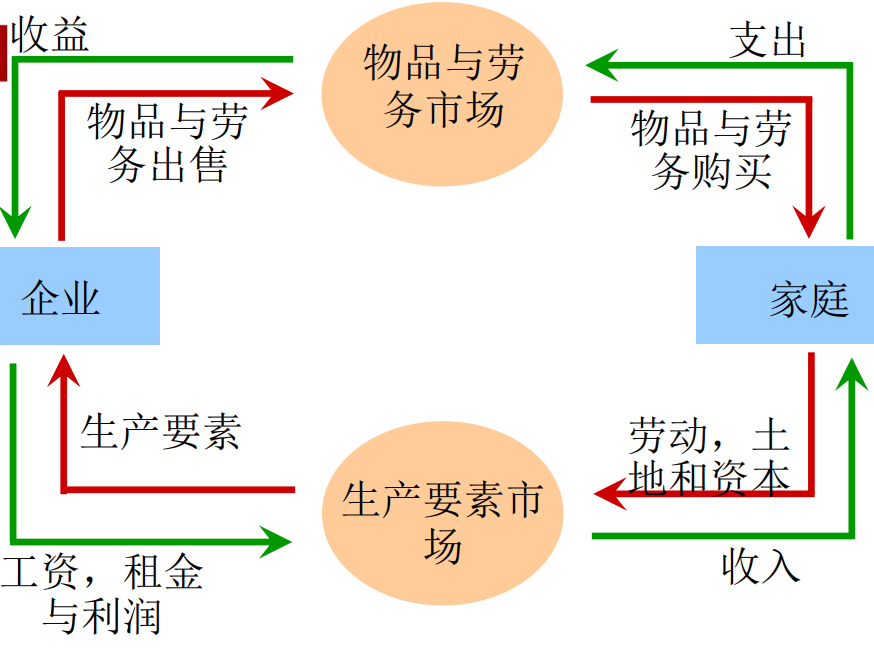
\includegraphics[width=0.4\textwidth]{循环流量图.png}
  \caption{循环流量图}
\end{figure}


% Chapter 2
\newpage
\section{贸易与比较优势}

\subsection{生产可能性边界}
生产可能性边界(Production Possibilities Frontier, PPF)表示在给定生产要素和技术条件下,一个经济体能够生产的两种产品的最大可能产量组合。

\textcolor{red}{机会成本}是指为了得到某件东西所必须放弃的其他东西的价值。例如,生产物品A所需的时间可以用来生产物品B的数量。

\begin{figure}[H] 
  \centering
  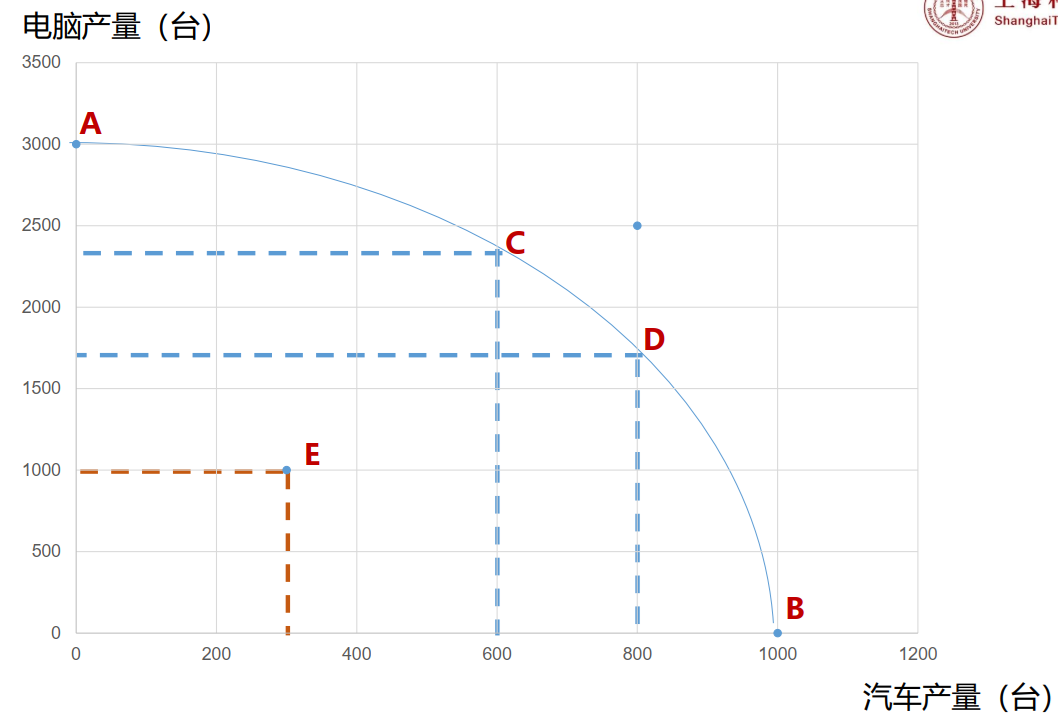
\includegraphics[width=0.8\textwidth]{生产可能性边界.png}
  \caption{生产可能性边界}
  \label{fig:ppf}
\end{figure}

生产可能性边界上的点代表生产效率最高的产量组合,即在这些点上,一种商品的增产只能通过减少另一种商品的产量来实现。边界内的点则表示资源没有得到充分利用,显示出生产效率较低。若PPF为直线,则表示两种商品之间的转换率是恒定的。

\subsection{比较优势与贸易}
\textcolor{red}{绝对优势}是指一个生产者在生产某种物品上使用的资源比其他生产者少。例如,美国生产1吨小麦只需10个劳动小时,而中国需要25个劳动小时,因此美国在生产小麦上拥有绝对优势。

\textcolor{red}{比较优势}指在所有生产活动中,具有相对较低机会成本的生产活动。比较优势说明了为什么即使一个国家在所有生产领域都没有绝对优势,仍然可以从贸易中获益。

例如,考虑以下机会成本:
\begin{itemize}
    \item 在美国,生产1台电脑的机会成本是10吨小麦,因为用于生产1台电脑的100劳动小时可以用来生产10吨小麦。
    \item 在中国,生产1台电脑的机会成本是5吨小麦,因为用于生产1台电脑的125劳动小时可以生产5吨小麦。
\end{itemize}

因此,中国在生产电脑上有比较优势。理论上,每个国家都应该专注于生产其具有比较优势的商品,然后通过贸易来获取其他商品,这样可以使得全球总产出最大化,提高所有参与国的经济福利。

\begin{figure}[H]
  \centering
  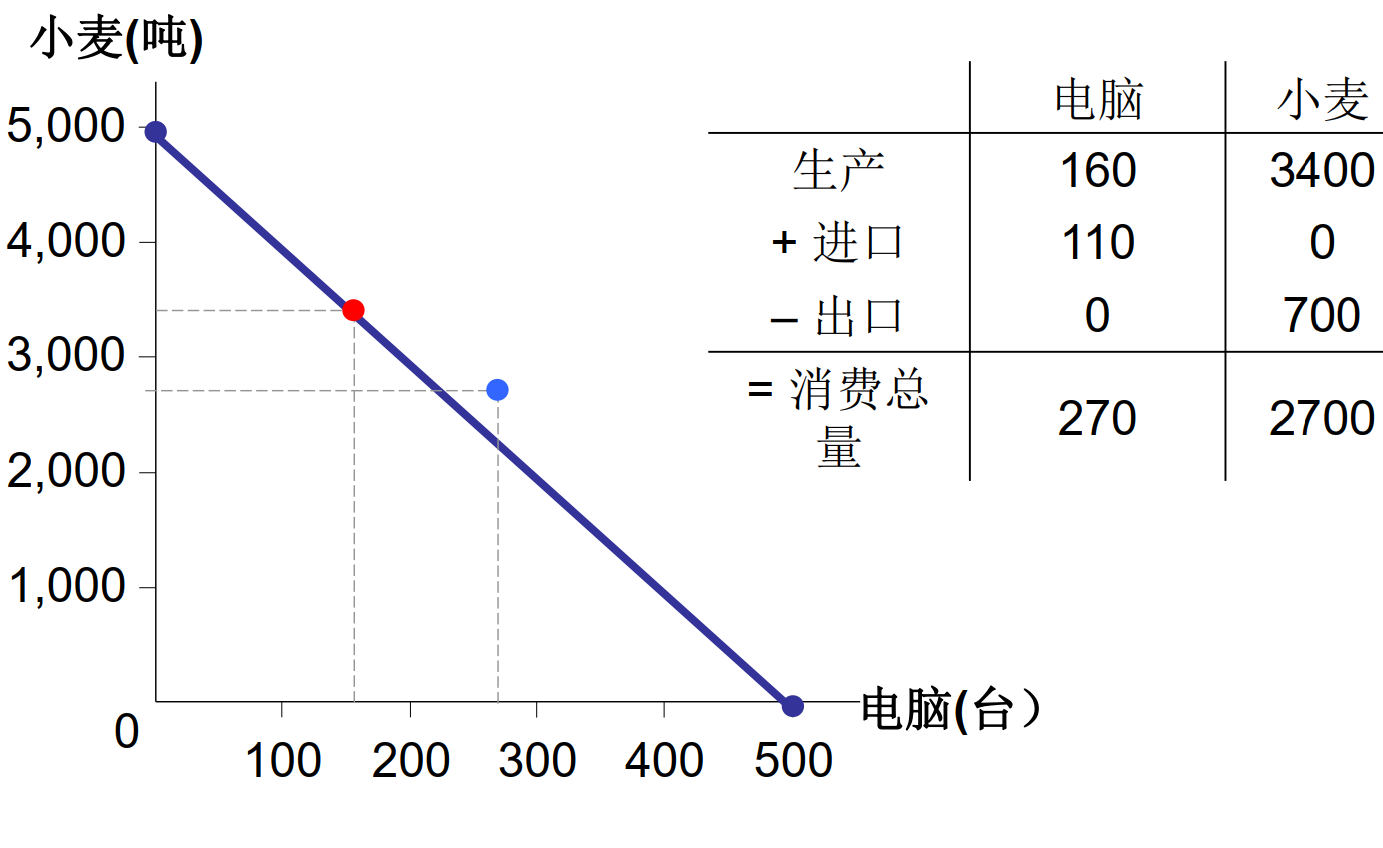
\includegraphics[width=0.4\textwidth]{贸易的好处.png}
  \caption{贸易的好处}
\end{figure}


% Chpter 3 供给与需求
\newpage
\section{供给与需求}
\setstretch{1.5}

\subsection{市场与竞争}
市场是由某种物品或服务的买者与卖者组成的一个群体;买者作为一个群体决定了需求,卖者作为一个群体决定了供给。

\textcolor{red}{完全竞争市场的特点}:
\begin{enumerate}
    \item 可供销售的物品是完全相同的
    \item 买者与卖者人数众多,以至于没有任何一个买者或卖者可以影响市场价格,也就是说,每个人都是“价格接受者” (price taker)
    \item 资源自由流动,市场信息畅通
\end{enumerate}

\subsection{需求与供给}

\subsubsection{需求(Demand)}
需求量(quantity demanded):买者愿意并且能够购买的一种物品的数量。需求定理(Law of Demand):在其他条件不变时,一种物品的价格上升,对该物品的需求量将减少 [价格可以看成机会成本]。市场需求是所有个人对某种特定物品或服务的需求的总和。

\subsubsection{需求曲线 (Demand Curve)}
需求表对应了需求曲线;根据习惯,我们让纵轴代表价格(P),横轴代表数量(Q)。

\begin{figure}[H]
  \centering
  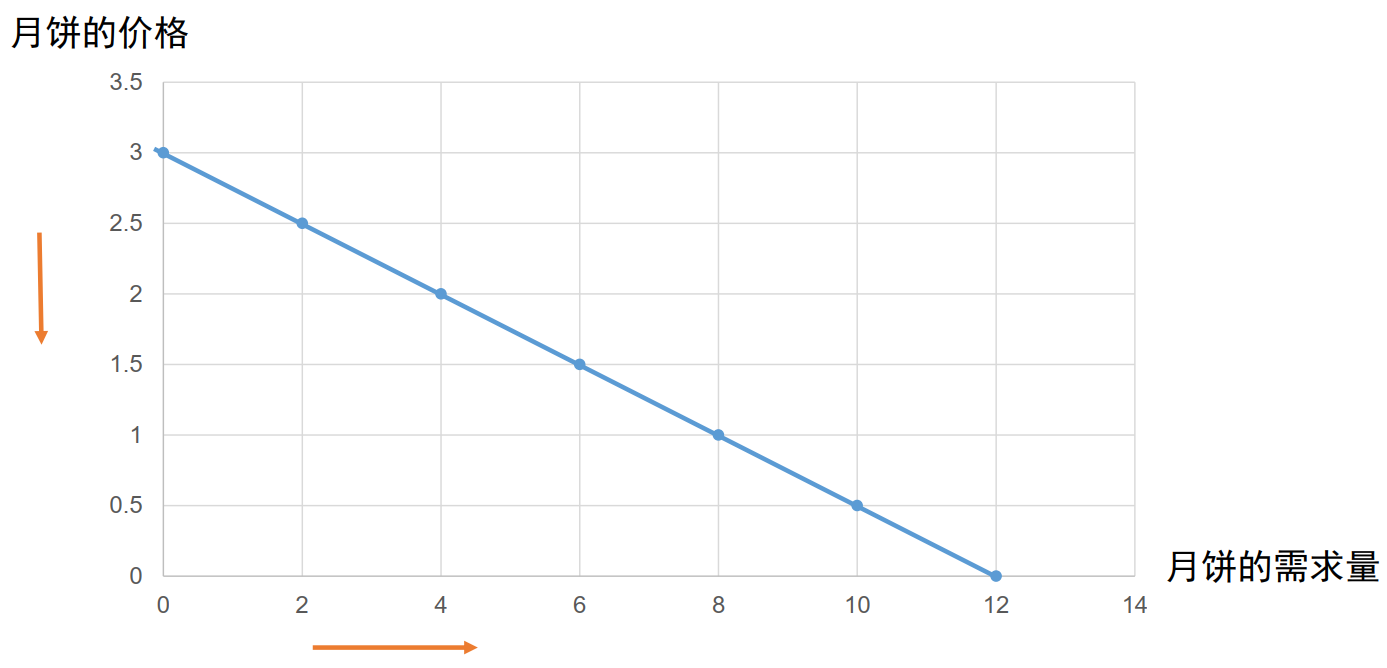
\includegraphics[width=0.6\textwidth]{需求曲线.png}
  \caption{需求曲线}
\end{figure}

需求曲线的移动:

\begin{figure}[H]
  \centering
  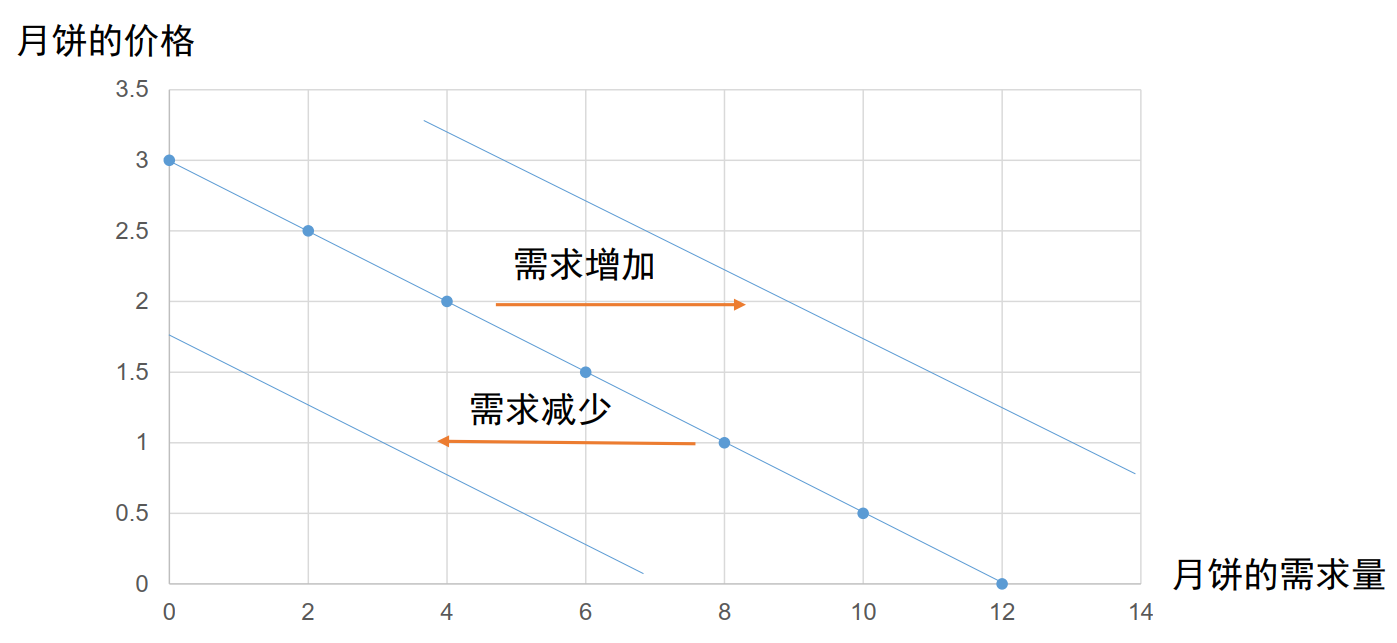
\includegraphics[width=0.6\textwidth]{需求曲线的移动.png}
  \caption{需求曲线的移动}
\end{figure}

引起需求曲线移动的因素:
\begin{enumerate}
    \item 收入的变化:收入降低意味着购买力减少,可能会减少某些物品的支出。
    \item 相关物品的价格变动:替代品和互补品的价格变动也会影响需求量。
    \item 偏好的变化:如流行趋势、健康意识等因素改变,会影响消费者对某些物品的需求。
    \item 预期未来的价格变动:如果预期未来价格上升,可能会提前购买。
    \item 买者数量的增减:买家的数量增加会增加总需求,数量减少则会降低总需求。
\end{enumerate}

\textcolor{red}{价格的变化不会引起需求曲线的变化。}价格变动只会引起沿着需求曲线的移动,而其他所有因素的影响表现为整条需求曲线的移动。

\subsubsection{供给 (Supply)}
供给量(quantity supplied):卖者愿意并且能够出售的该种物品的数量。

供给定理(Law of Supply):在其他条件不变时,一种物品价格上升,该物品供给量将增加。

\subsubsection{供给曲线 (Supply Curve)}
供给表对应了供给曲线;根据习惯,我们让纵轴代表价格(P),横轴代表数量(Q)。

\begin{figure}[H]
  \centering
  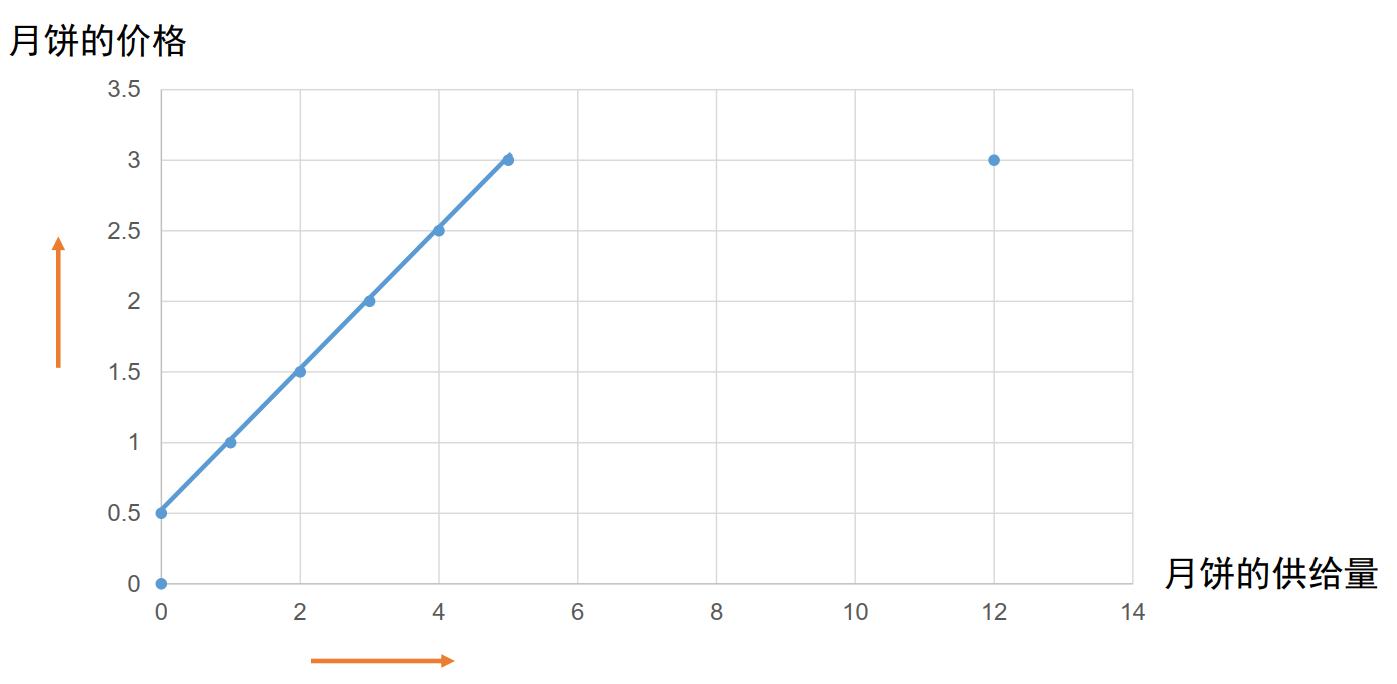
\includegraphics[width=0.6\textwidth]{供给曲线.png}
  \caption{供给曲线}
\end{figure}

供给曲线的移动:

\begin{figure}[H]
  \centering
  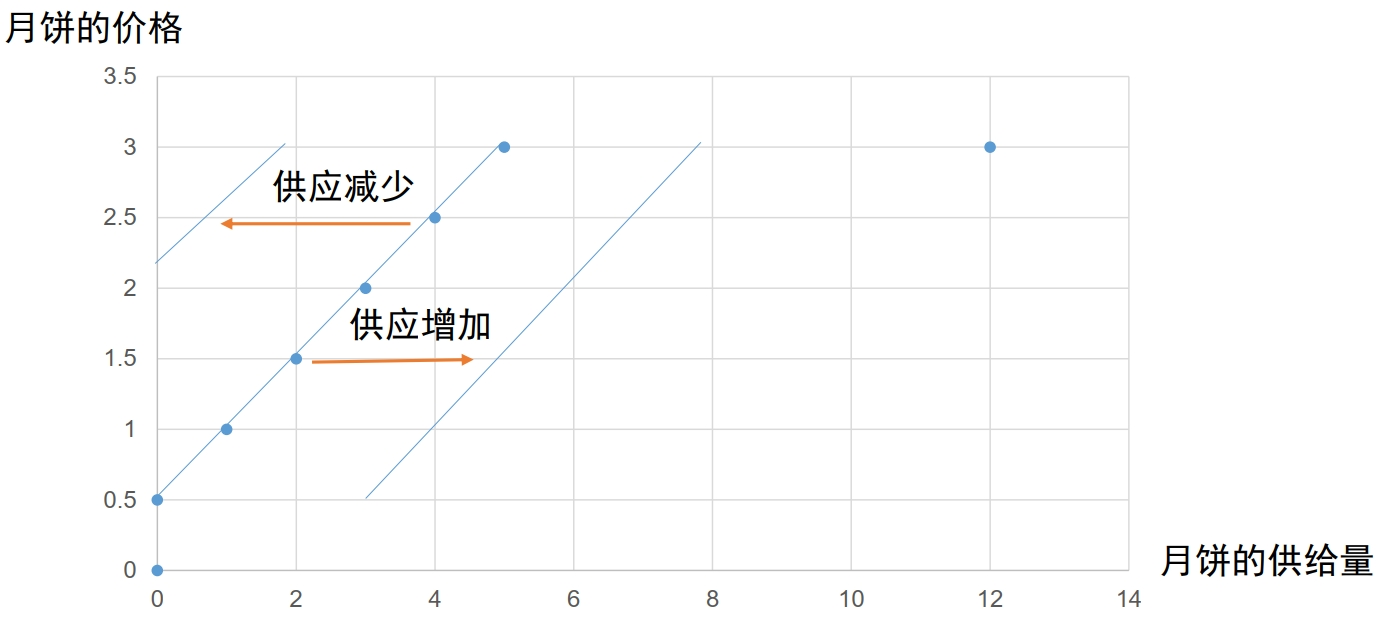
\includegraphics[width=0.6\textwidth]{供给曲线的移动.png}
  \caption{供给曲线的移动}
\end{figure}

引起供给曲线移动的因素:
\begin{enumerate}
    \item 投入品价格的变动:如原材料成本上升会减少供给。
    \item 生产技术的改进:如技术进步通常会增加供给。
    \item 生产者对未来价格的预期:如预期价格上升可能会暂时减少供给以备未来出售。
    \item 卖者数量的增减:卖家数量增加会增加市场供给,数量减少会减少市场供给。
\end{enumerate}

\textcolor{red}{价格的变化不会引起供给曲线的变化。}价格变动引起沿着供给曲线的移动,而其他因素影响供给曲线的整体移动。

\subsubsection{供给与需求的均衡}
市场的供给曲线与需求曲线交汇于一点,这一点被称为市场的均衡。

\textcolor{red}{均衡(equilibrium)}:市场价格达到使供给量与需求量相等的状态。

\noindent 市场均衡时的价格称为均衡价格(equilibrium price),均衡数量称为均衡数量(equilibrium quantity)。均衡价格有时也被称为市场出清价格(clearing price)。

\begin{figure}[H]
  \centering
  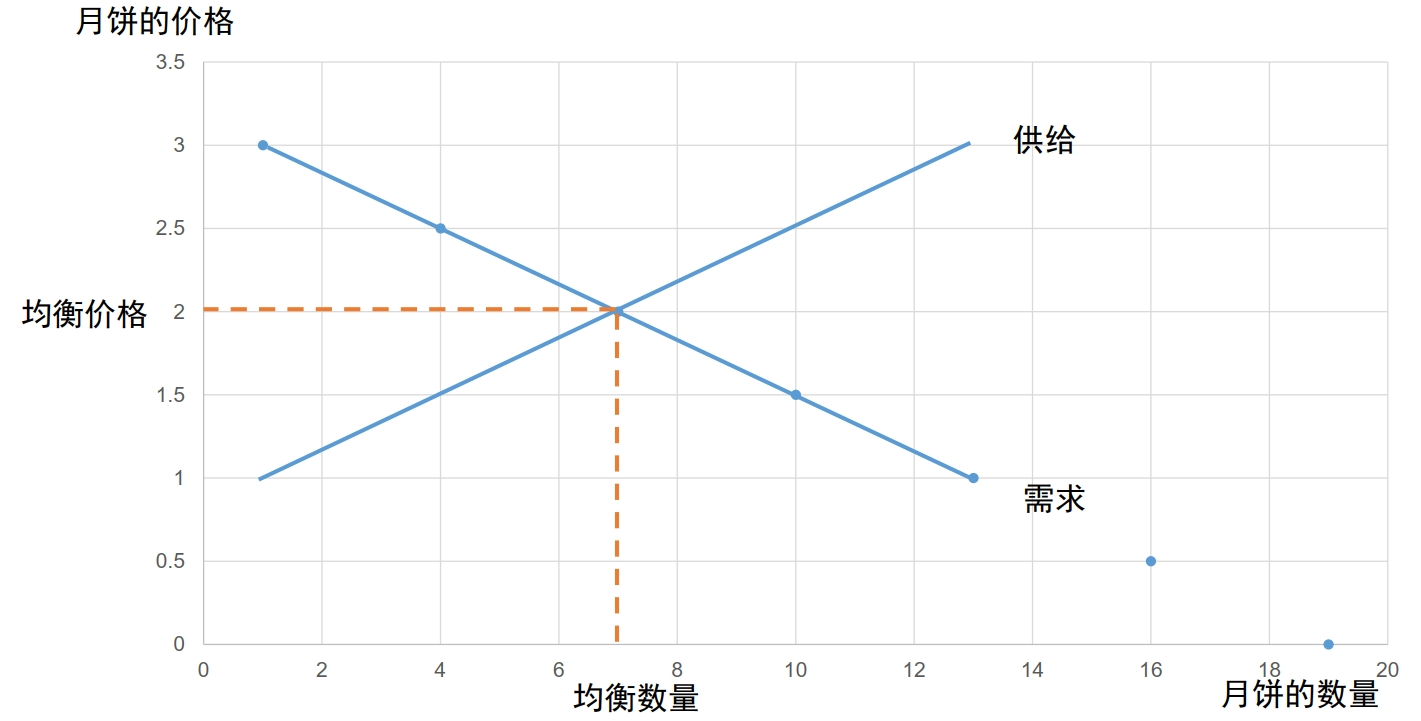
\includegraphics[width=0.6\textwidth]{均衡.png}
  \caption{市场均衡}
\end{figure}

市场自然而然地向均衡靠拢:过剩情况下,卖家通过降价增加销量,短缺时通过涨价减少需求。

\subsubsection{分析均衡的变动}
分析均衡变动的步骤:
\begin{enumerate}
    \item 确定事件是影响供给还是需求(或两者)。
    \item 确定曲线移动的方向。
    \item 使用供求图说明这种变动如何改变均衡价格和数量。
\end{enumerate}

示例分析:汽油价格上升与新技术降低生产成本。

\begin{figure}[H]
  \centering
  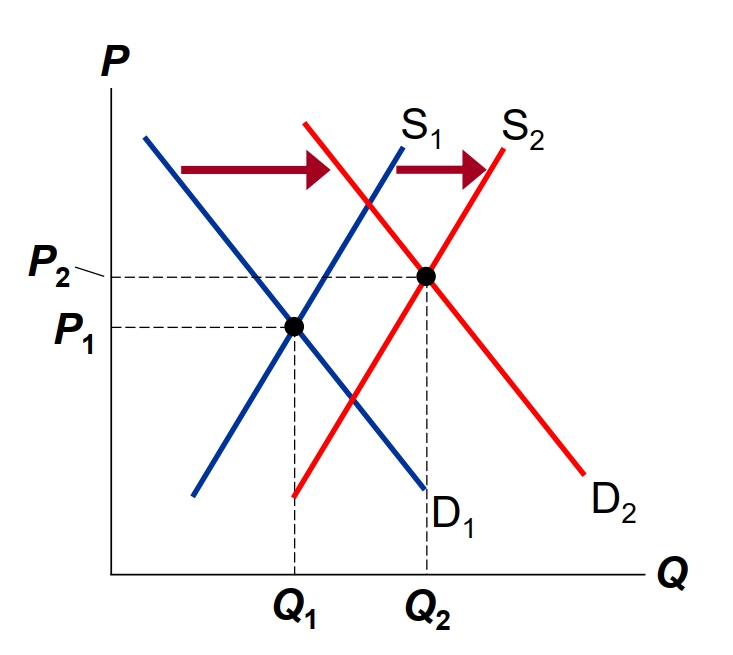
\includegraphics[width=0.4\textwidth]{均衡分析.png}
  \caption{均衡分析}
\end{figure}

\subsection{弹性}

\subsubsection{需求价格弹性}
\textcolor{red}{需求价格弹性(price elasticity of demand)}衡量需求量对价格变动的反应程度。

\[ E_d = \left| \frac{\Delta Q / Q}{\Delta P / P} \right| = \left| \frac{\Delta Q}{\Delta P} \cdot \frac{P}{Q} \right| \]

\textcolor{red}{中点法求弹性}计算一段需求曲线上两点间的平均弹性。

\[ E_d = \frac{\frac{Q_2 - Q_1}{\frac{Q_2 + Q_1}{2}}}{\frac{P_2 - P_1}{\frac{P_2 + P_1}{2}}} \]

\textcolor{red}{点价格弹性}测量特定点上需求量对价格变化的敏感度。

\[ E_d = \frac{dQ}{dP} \times \frac{P}{Q} \]

线性需求曲线的弹性:

\[ E_d = \frac{dQ}{dP} \times \frac{P}{Q} = -b \times \frac{P}{Q} \]

这里,$-b$ 是需求曲线的斜率,而 $\frac{P}{Q}$ 是给定点上的价格与需求量的比率。

需求价格弹性的决定因素:
\begin{itemize}
  \item 当价格很高,需求量很低时(即在需求曲线的左上方),$\frac{P}{Q}$ 的值较大,这使得弹性的绝对值大于 1,表明需求在这一区域是弹性的。
  \item 当价格降低,需求量增加时(即在需求曲线的右下方),$\frac{P}{Q}$ 的值减小,弹性的绝对值也随之减小,需求变得更加无弹性。
  \item 在需求曲线的中点,弹性的绝对值正好等于 1,这个点称为单位弹性点。
\end{itemize}

弹性大于1时需求富有弹性,小于1时缺乏弹性,等于1时具有单位弹性。

\begin{figure}[H]
  \centering
  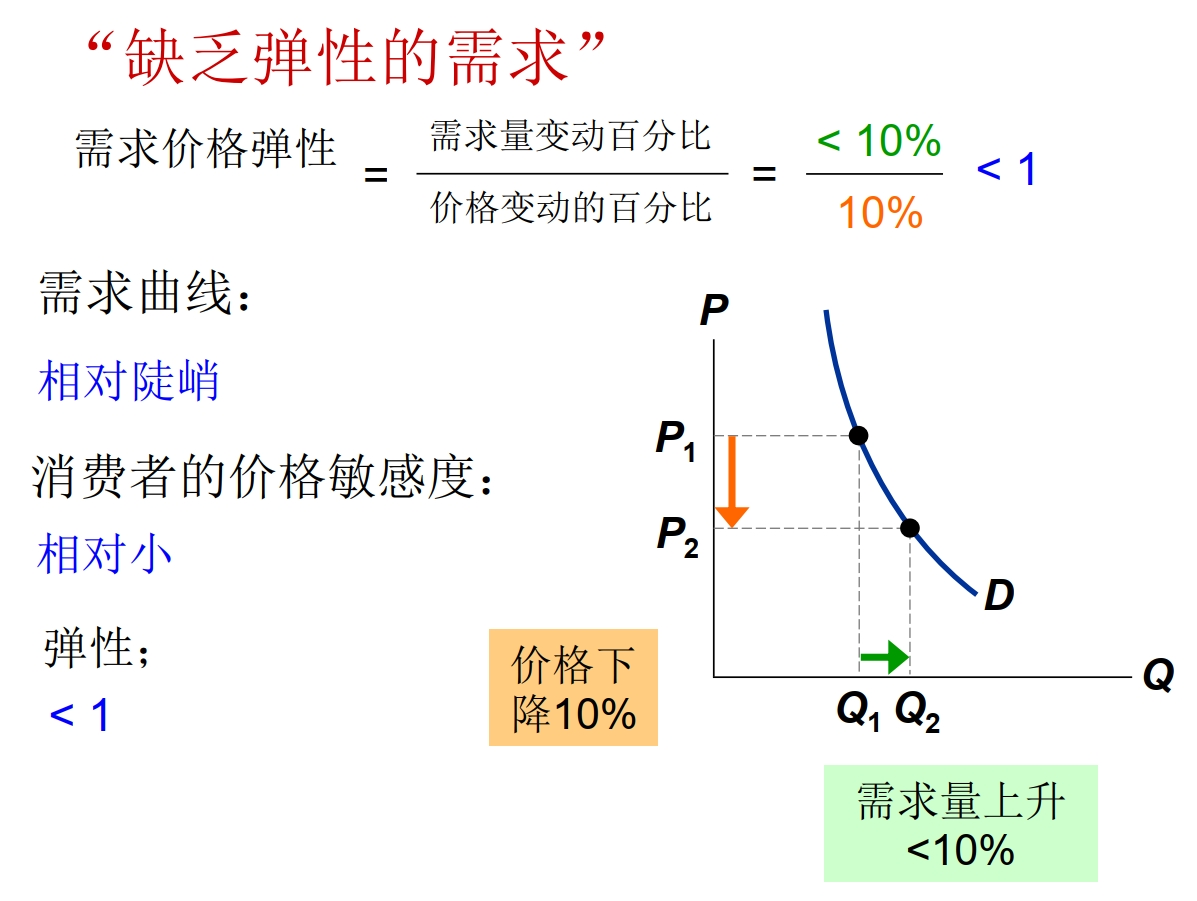
\includegraphics[width=0.6\textwidth]{缺乏弹性的需求.png}
  \caption{缺乏弹性的需求}
\end{figure}

\begin{figure}[H]
  \centering
  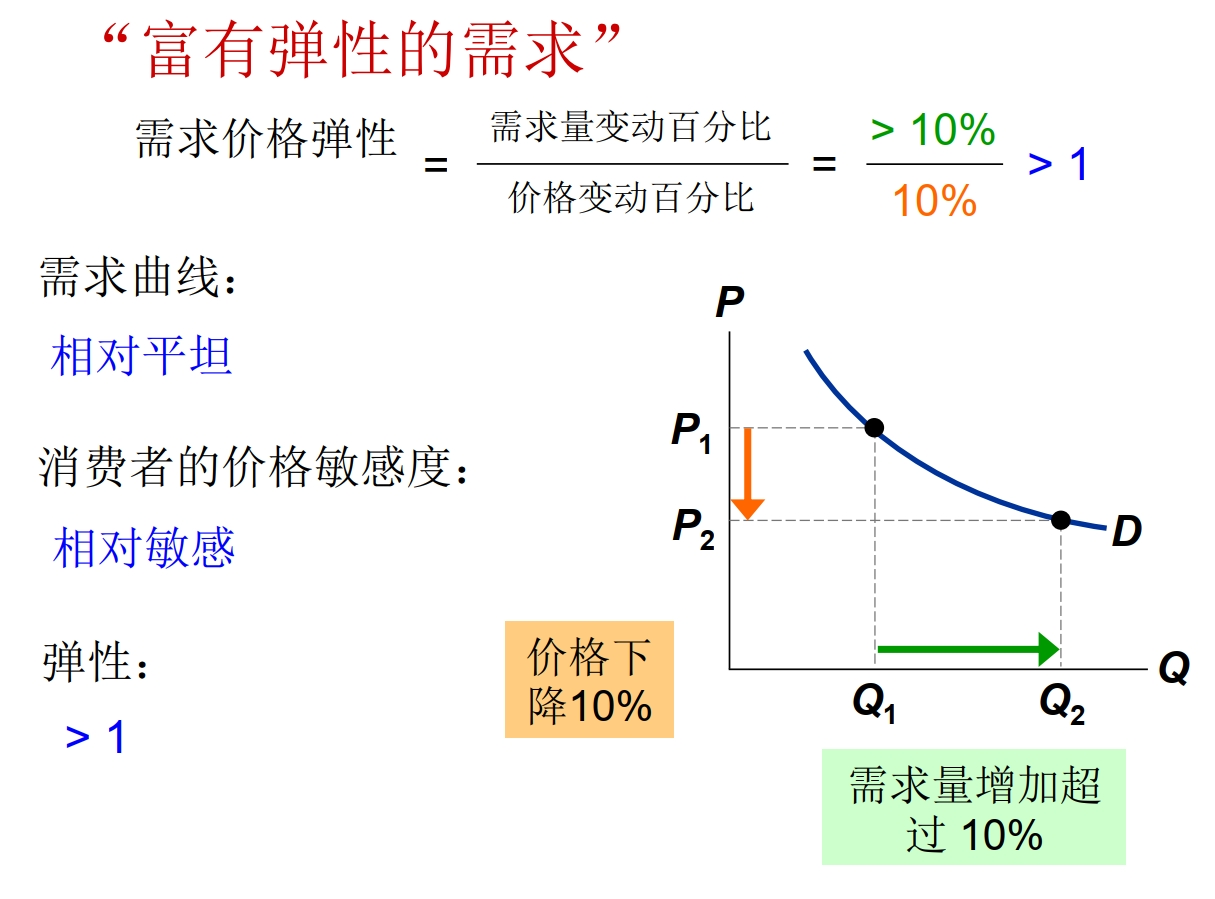
\includegraphics[width=0.6\textwidth]{富有弹性的需求.png}
  \caption{富有弹性的需求}
\end{figure}

\textcolor{red}{其他需求弹性}包括需求收入弹性和需求的交叉价格弹性。

\textcolor{red}{需求收入弹性(income elasticity of demand)}:衡量消费者收入变动时需求量如何变动。正常物品的需求收入弹性为正数,而低档物品的为负数
$$E_{i} = \frac{\Delta Q / Q}{\Delta I / I}$$
$$E_{i} = \frac{dQ / Q}{dI / I}$$

\textcolor{red}{需求的交叉价格弹性}:替代品的交叉价格弹性为正数,互补品的交叉价格弹性为负数
$$E_{xy} = \frac{\Delta Q_x / Q_x}{\Delta P_y / P_y}$$
$$E_{xy} = \frac{dQ_x / Q_x}{dP_y / P_y}$$

\subsubsection{供给价格弹性与供给曲线}
\textcolor{red}{供给价格弹性(price elasticity of supply)}衡量供给量对价格变动的反应程度。

供给价格弹性的决定因素包括卖者调整生产量的灵活性和时间范围(长期供给的价格弹性都要大于短期供给的价格弹性)。


% Chapter 4
\newpage
\section{税收与政府政策}
\setstretch{1.5}

\subsection{价格控制}

\subsubsection{价格上限 (price ceiling)}
价格上限是指出售一种物品或服务的法定最高价格。当价格上限设定在低于市场均衡价格时,会造成供不应求的局面,导致短缺。

\begin{figure}[H] 
  \centering
  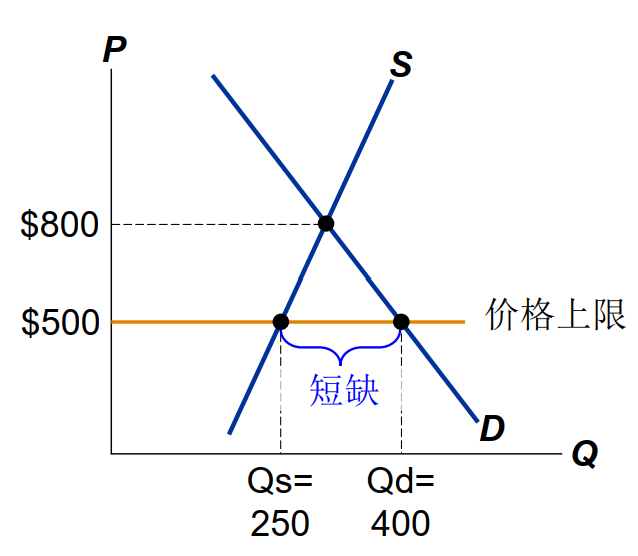
\includegraphics[width=0.4\textwidth]{价格上限.png}
  \caption{价格上限}
\end{figure}

\subsubsection{价格下限 (price floor)}
价格下限是出售一种物品或服务的法定最低价格。例如,最低工资法和最低粮食价格保护。当价格下限设定在高于市场均衡价格时,会造成供过于求,导致过剩,例如失业。

\begin{figure}[H] 
  \centering
  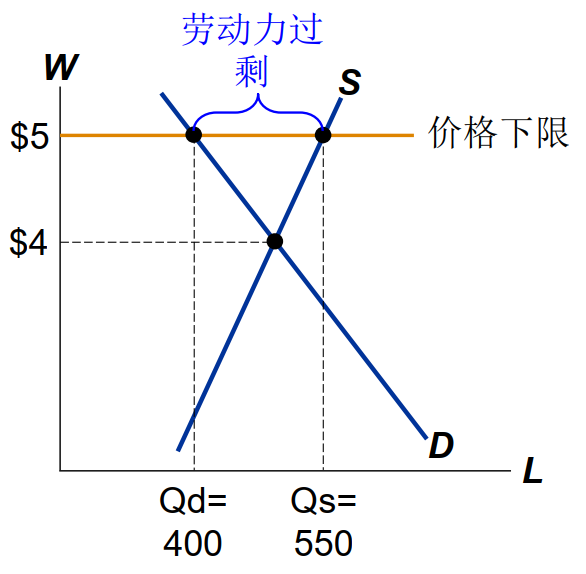
\includegraphics[width=0.4\textwidth]{价格下限.png}
  \caption{价格下限}
\end{figure}

\textcolor{red}{价格下限和价格上限对市场造成的影响是重要的分析课题。}

\newpage

\subsection{税收}
不管税收是施加在买家还是卖家身上,其影响对市场来说是一样的。税收会在买家支付的价格和卖家接收的价格之间形成一个楔形,提高买家支付的价格,降低卖家接收的价格,从而减少市场上的交易量。

\begin{figure}[H] 
  \centering
  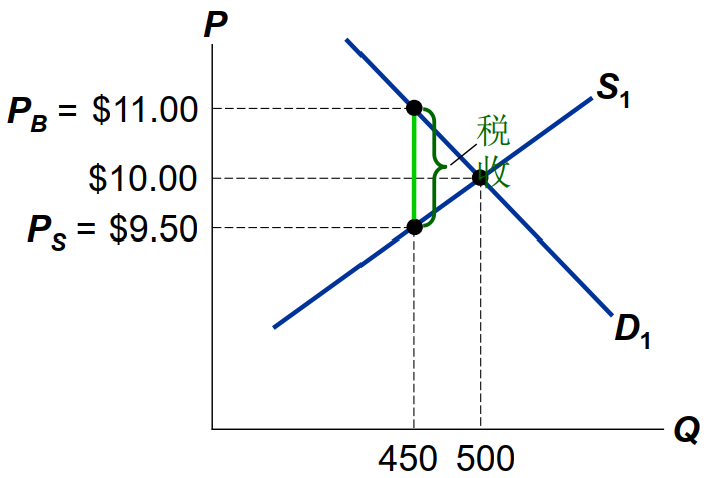
\includegraphics[width=0.4\textwidth]{税收.png}
  \caption{税收}
\end{figure}

\subsubsection{练习题}
假设市场的供给和需求方程如下所描述:
\[ Q_s = 2P \]
\[ Q_d = 300 - P \]

a. 若对买家征收定额税T,新的需求方程是什么?
b. 新的市场均衡数量是多少?买家和卖家的税收负担各是多少?

% a. 新的需求方程
原需求方程为: 
\[ Q_d = 300 - P \]

新的需求方程为: 
\[ Q'_d = 300 - (P + T) \]

% b. 新的市场均衡数量及税收负担
要找到新的市场均衡,我们设供给等于需求:
\[ Q_s = Q'_d \]
代入供给方程和新的需求方程:
\[ 2P = 300 - P - T \]
解这个方程可得新的均衡价格 \( P_s^* = 100 - \frac{T}{3} \)。

将 \( P_s^* \) 代入任一方程式中(供给或需求)得到新的市场均衡数量 \( Q^* = 200 - \frac{2T}{3} \)。即 \( P_d = 100 + \frac{2T}{3} \)。

税前均衡价格由原供需方程确定:
\[ 2P_0 = 300 - P_0 \]
\[ P_0 = 100 \]

所以,买家承担的税收负担是 \( \frac{2T}{3} \),而卖家承担的是 \( \frac{T}{3} \)。







% Chapter 5
\newpage
\section{福利经济学}
\setstretch{1.5}
\textcolor{red}{福利经济学(welfare economics)}研究资源配置如何影响经济福利的一门学问。

我们从考察买者和卖者的利益开始,然后考虑如何可以使所有人的利益最大化。最终我们将得出一个意义深远的结论:市场上的供求均衡可以最大化买者和卖者的总利益 [市场通常是组织经济活动的一种好方法]。

%5.1
\subsection{买者的利益:消费者剩余}
\textcolor{red}{支付意愿}是买者愿意为某种物品支付的最高金额,代表了买者对于该物品的评价(valuation)。

\begin{figure}[H]
  \centering
  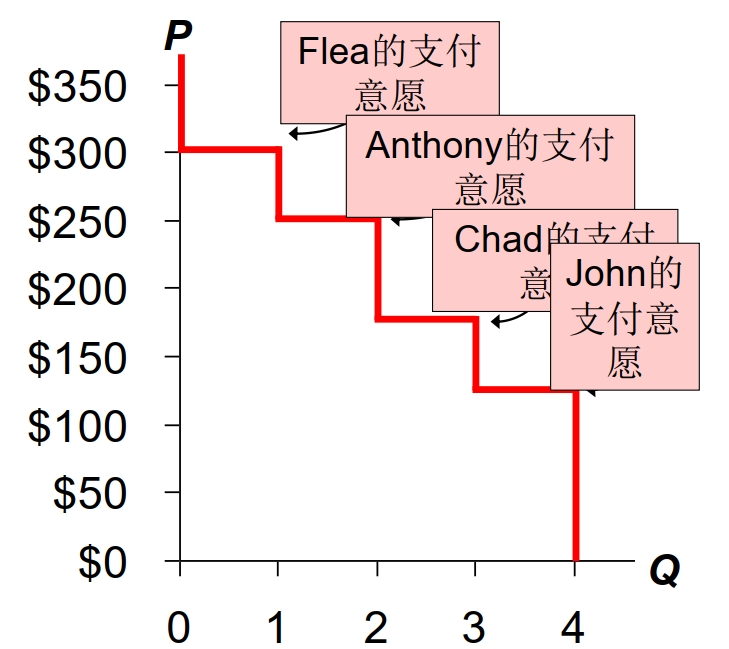
\includegraphics[width=0.4\textwidth]{支付意愿.png}
  \caption{支付意愿}
\end{figure}

在任意数量上,需求曲线的高度代表边界买者的支付意愿。

\textcolor{red}{边际买者}是指如果价格再提高一点就首先离开市场的买者。

\textcolor{red}{消费者剩余}是买者愿意为一种物品支付的量减去其为此实际支付的量。
\[
\text{消费者剩余} = \int_{P}^{P_{\text{最大}}} D(P) \, dP - Q \cdot P
\]
\textcolor{red}{总消费者剩余}是所有消费者剩余之和,等于需求曲线以下,价格之上的面积。
\[
\text{总消费者剩余} = \int_{0}^{Q} P_{\text{d}}(q) \, dq - P \cdot Q
\]

\begin{figure}[H]
  \centering
  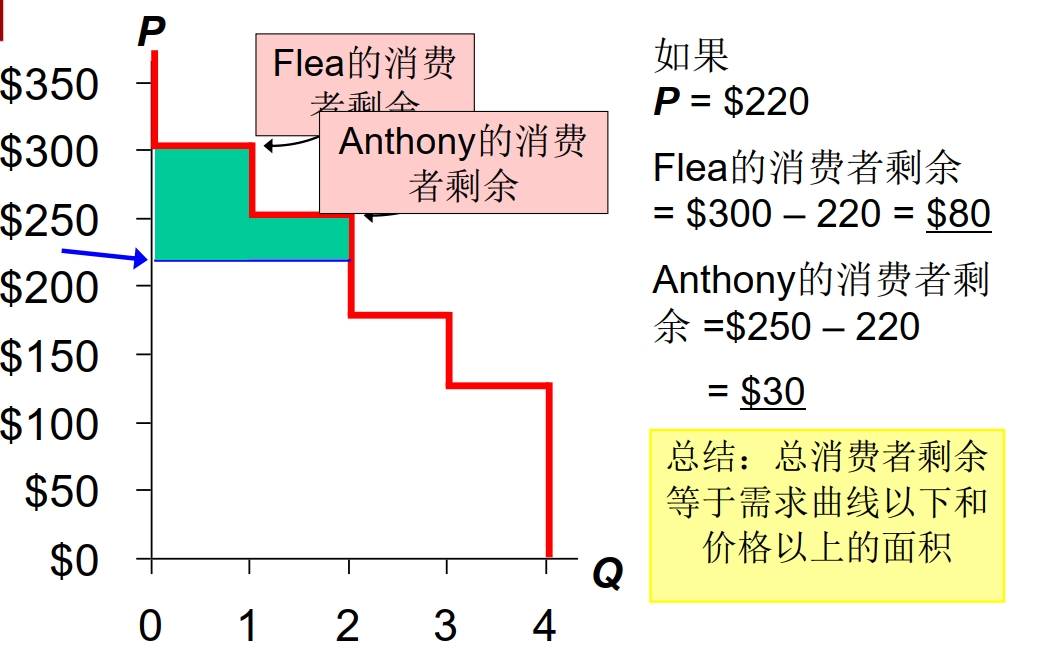
\includegraphics[width=0.6\textwidth]{消费者剩余.png}
  \caption{消费者剩余}
\end{figure}

大量买者的需求曲线与消费者剩余。

\begin{figure}[H]
  \centering
  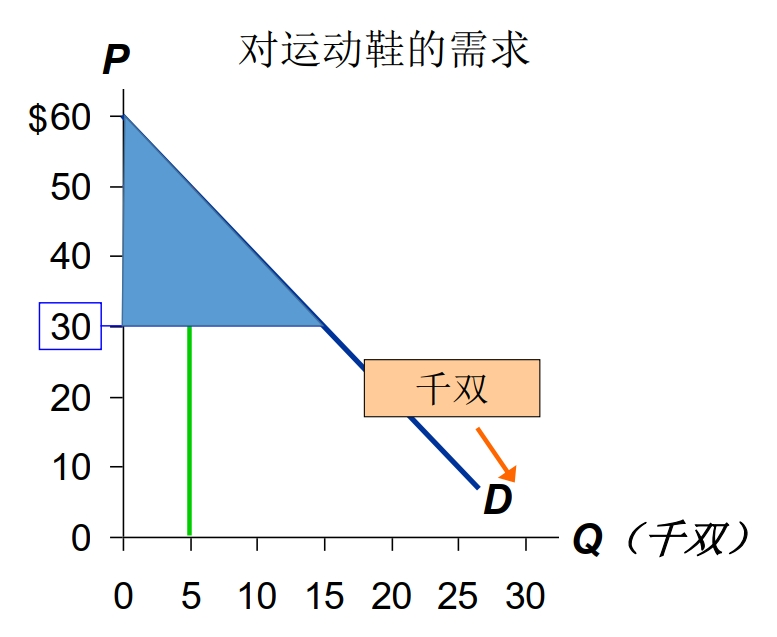
\includegraphics[width=0.4\textwidth]{大量买者的消费者剩余.png}
  \caption{大量买者的消费者剩余}
\end{figure}

例如,假设某个市场的需求为一直线,计算消费者剩余的公式可以是:
\[
S = \frac{1}{2} \times (15 - 0) \times (60 - 30)
\]

更高的价格会减少消费者剩余。

\begin{figure}[H]
  \centering
  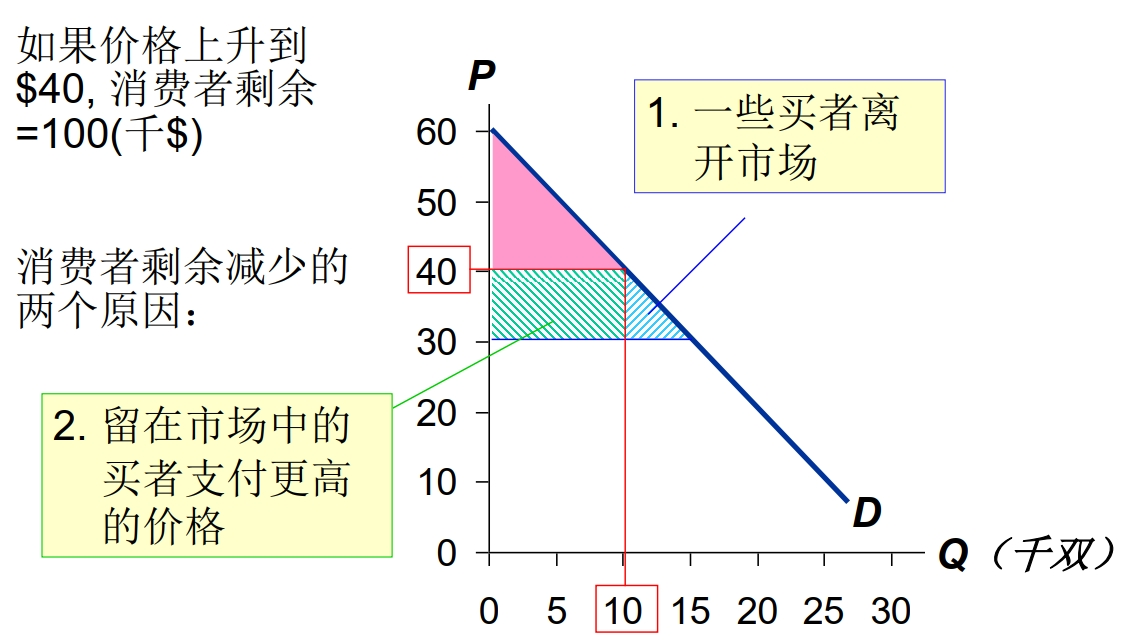
\includegraphics[width=0.6\textwidth]{更高的价格会减少消费者剩余.png}
  \caption{更高的价格会减少消费者剩余}
\end{figure}

%5.2
\subsection{卖者的利益:生产者剩余}

\textcolor{red}{成本}是卖者为了生产一种物品而必须放弃的所有东西的价值。实际上是机会成本:包括所有用于生产物品的资源的成本和卖者对于他们自己时间、精力的评价。一个卖者生产和出售物品或服务,除非价格高于他或她的成本。因此,成本衡量了出售意愿。

\subsubsection{成本与供给曲线}

\begin{figure}[H]
  \centering
  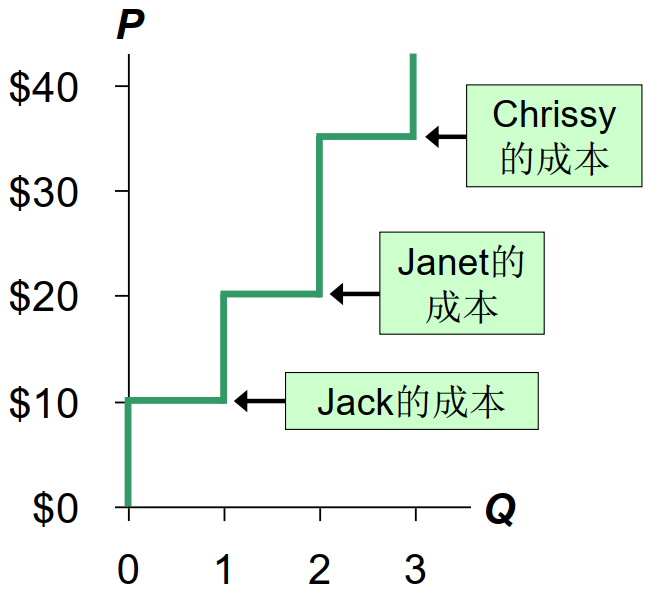
\includegraphics[width=0.4\textwidth]{成本与供给曲线.png}
  \caption{成本与供给曲线}
\end{figure}

在每个数量,供给曲线的高度是边际卖者的成本。

\textcolor{red}{边际卖者}是如果价格再低一点就首先离开市场的卖者。

\subsubsection{生产者剩余与供给曲线}

\textcolor{red}{生产者剩余}是出售价格减去其生产成本。
生产者剩余 = 价格 - 成本。
总生产者剩余等于价格以下和供给曲线以上的面积。

\begin{figure}[H]
  \centering
  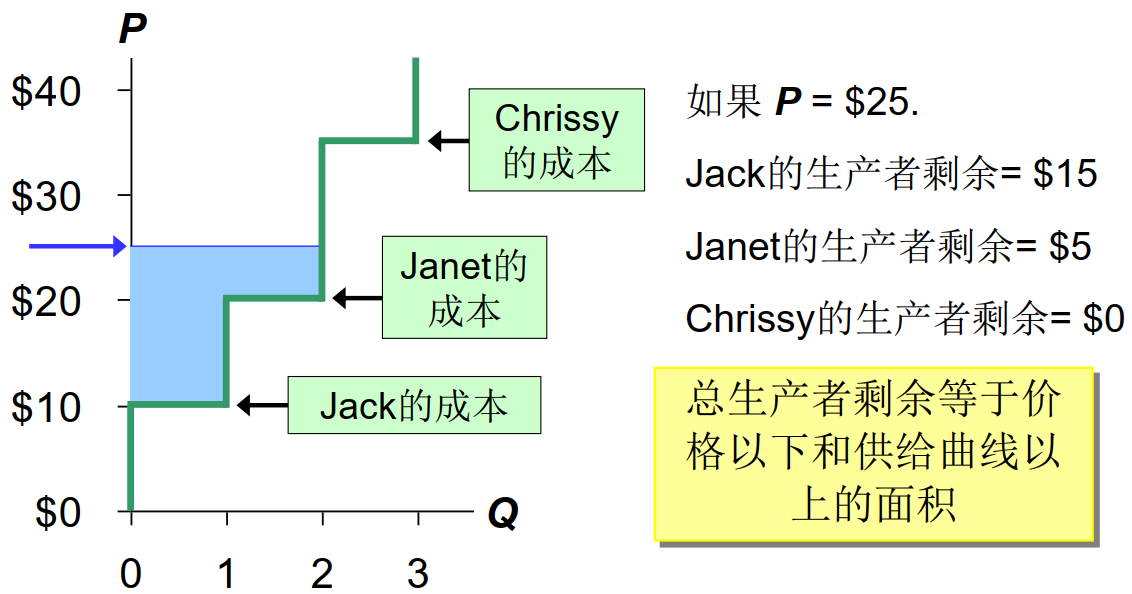
\includegraphics[width=0.6\textwidth]{生产者剩余与供给曲线.png}
  \caption{生产者剩余与供给曲线}
\end{figure}

大量卖者的生产者剩余。

\begin{figure}[H]
  \centering
  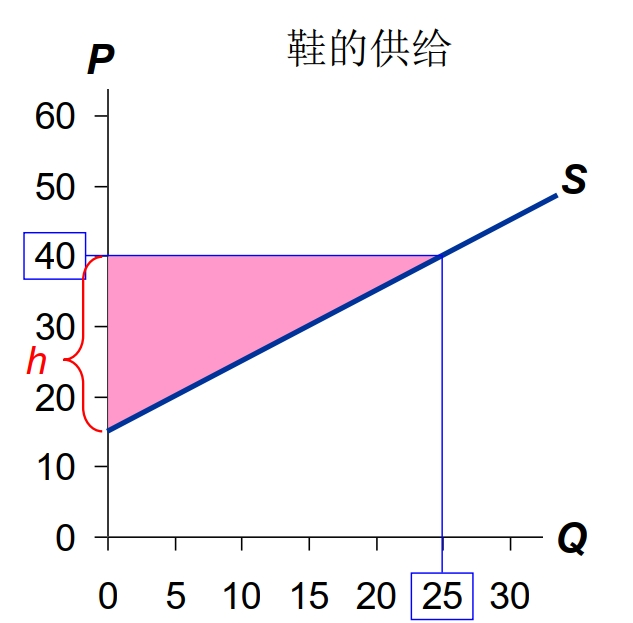
\includegraphics[width=0.4\textwidth]{大量卖者的生产者剩余.png}
  \caption{大量卖者的生产者剩余}
\end{figure}

\textcolor{red}{总生产者剩余}是所有生产者剩余之和,等于供给曲线以上,价格以下的面积。
\[
S = \frac{1}{2} \times (25 - 0) \times (40 - 15)
\]

更低的价格将减少生产者剩余。

\begin{figure}[H]
  \centering
  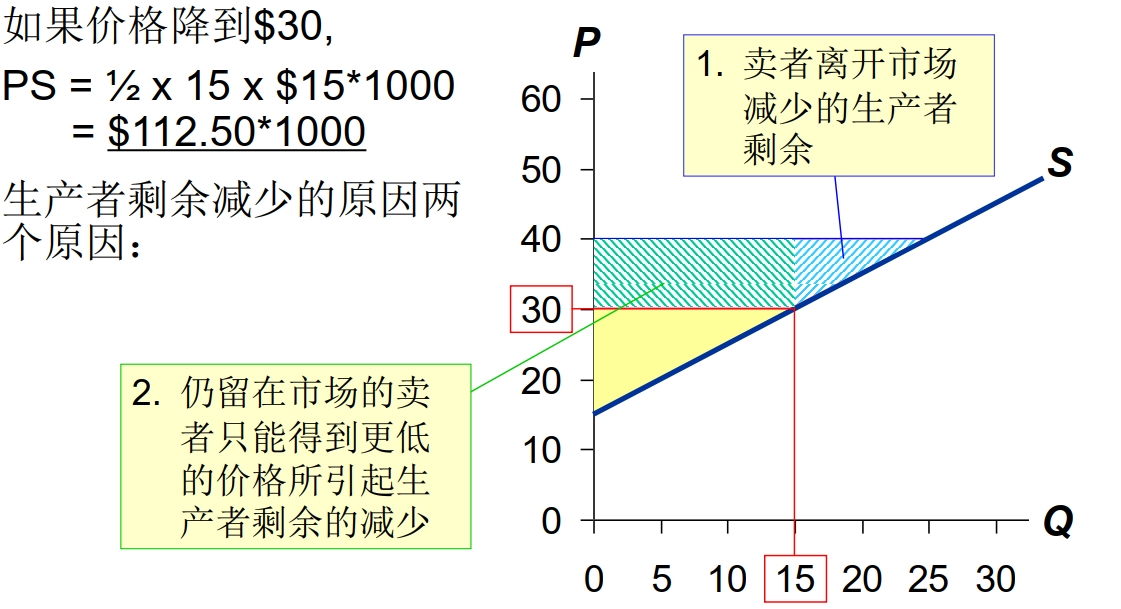
\includegraphics[width=0.6\textwidth]{更低价格的生产者剩余.png}
  \caption{更低价格的生产者剩余}
\end{figure}

%5.3
\subsection{市场效率(市场总福利)}
市场总剩余(总福利)= CS (consumer supply) +  PS (producer supply) 
= (买者的评价) - (买者支付的量) + (卖者得到的量) - (卖者的成本) 
= (买者的评价) - (卖者的成本) 
= (买者+卖者)参与市场贸易得到的总收益。

如果资源配置使总剩余最大化,那我们可以说,这种配置是有效率的。

\begin{figure}[H]
  \centering
  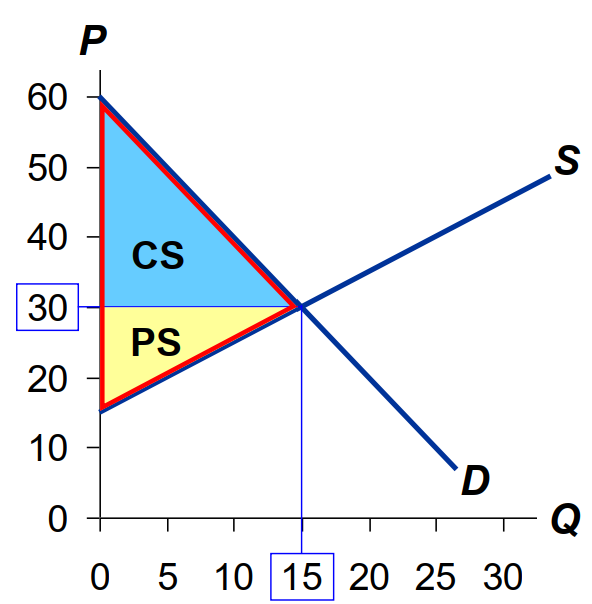
\includegraphics[width=0.4\textwidth]{市场总福利.png}
  \caption{市场均衡时的市场总福利}
\end{figure}

当市场均衡时,市场总剩余最大;高于均衡的数量会使总剩余减少;低于均衡的数量会使总剩余减少。

市场均衡配置是最有效的配置。市场均衡产量使总剩余最大:在其他任何数量下,向市场均衡数量移动都能使总剩余增加。

\subsection{税收的代价}
税收的无谓损失是市场扭曲(例如税收)引起总剩余减少的部分。由于税收,在QT与QE单位之间的物品没有被售出。

\begin{figure}[H]
  \centering
  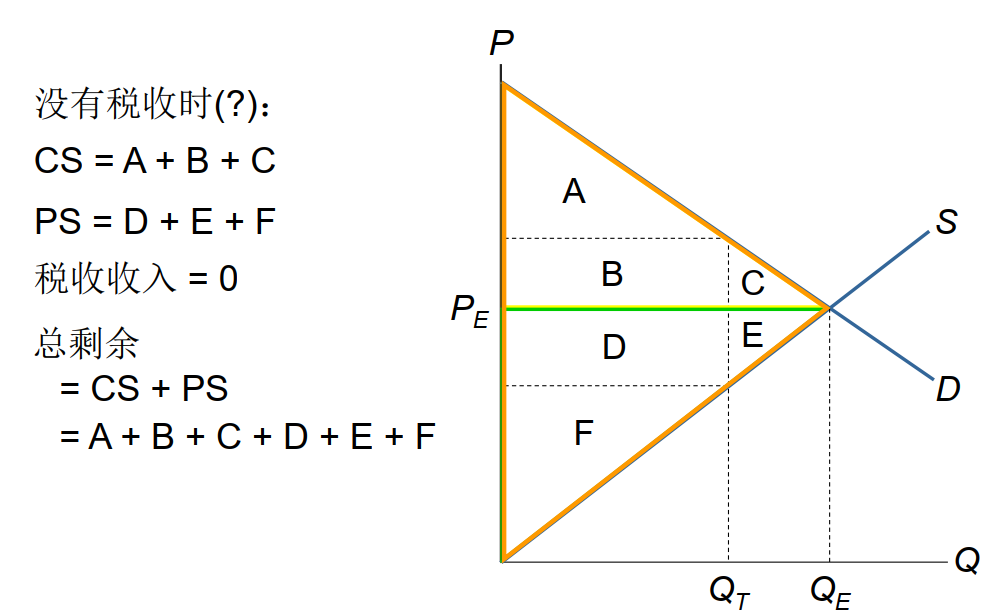
\includegraphics[width=0.6\textwidth]{没有税收时的总福利.png}
  \caption{没有税收时的总福利}
\end{figure}

\begin{figure}[H]
  \centering
  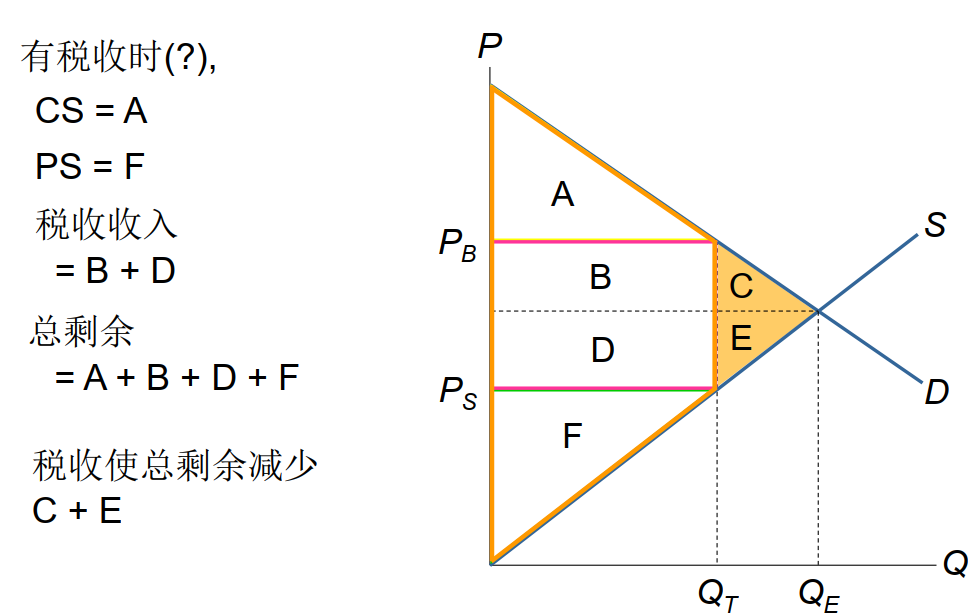
\includegraphics[width=0.6\textwidth]{有税收时的总福利.png}
  \caption{有税收时的总福利}
\end{figure}

C与E被称为税收的无谓损失(deadweight loss)。决定无谓损失大小的因素之一是弹性。弹性越小,无谓损失越小。


\begin{figure}[H] 
  \centering % 使图片居中显示
  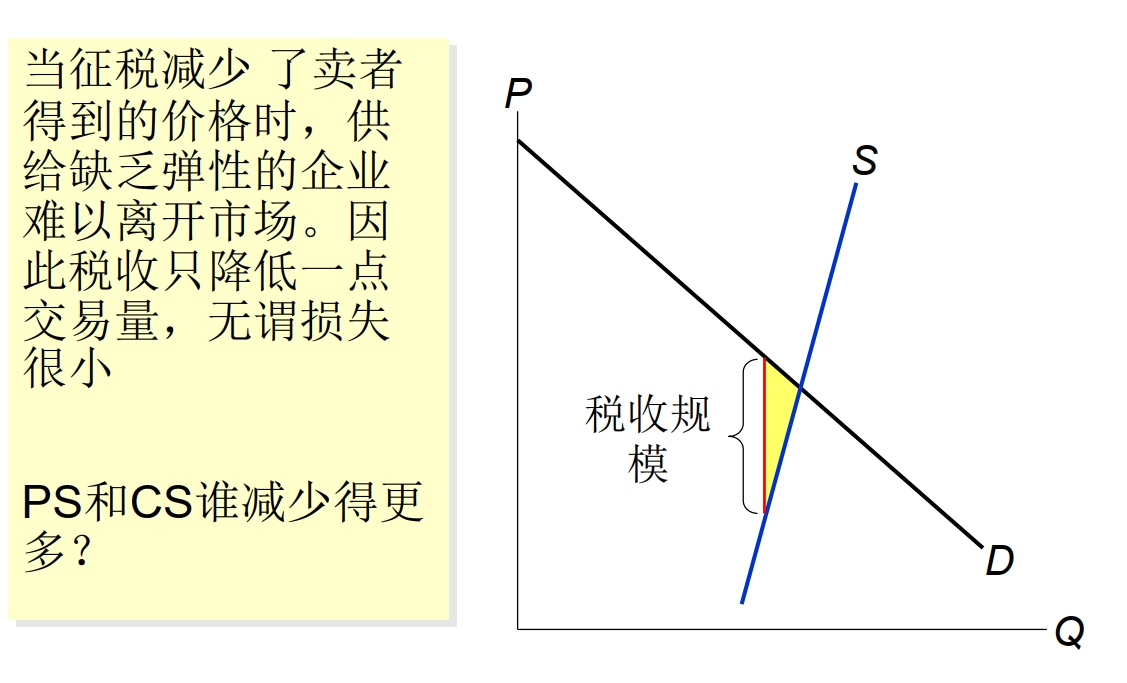
\includegraphics[width=0.5\textwidth]{弹性小,无谓损失小.png} 
  \caption{弹性小,无谓损失小} % 为图片添加标题
\end{figure}
\begin{figure}[H] 
  \centering % 使图片居中显示
  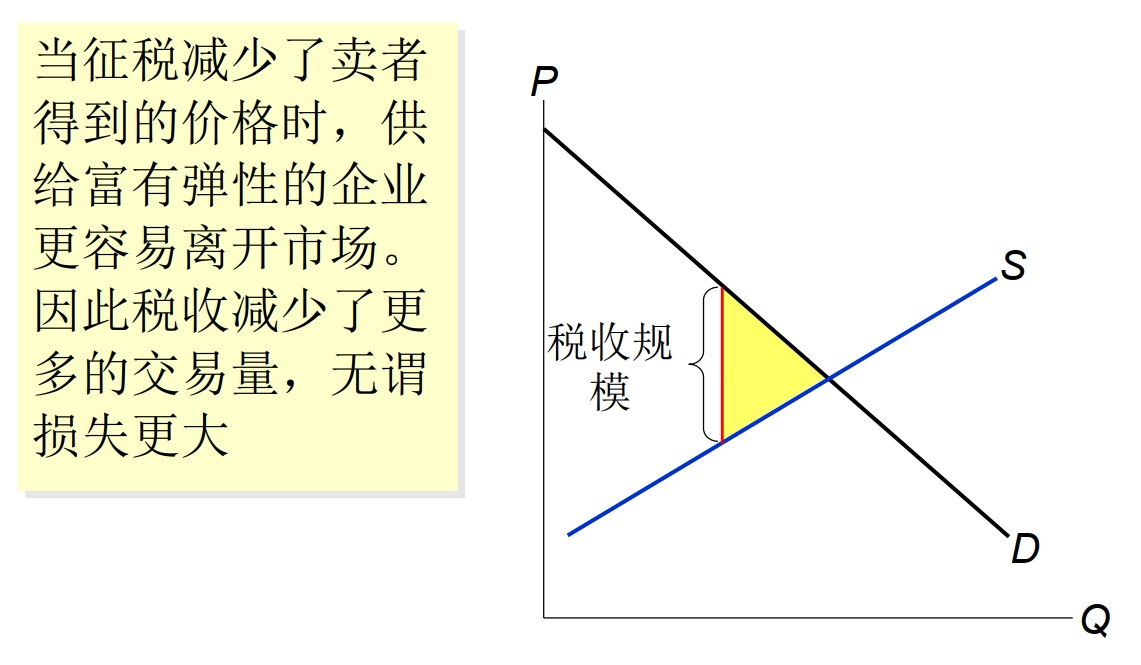
\includegraphics[width=0.5\textwidth]{弹性大,无谓损失大.png} 
  \caption{弹性大,无谓损失大} % 为图片添加标题
\end{figure}

税收规模增长速度比无谓损失的增长速度小
\begin{figure}[H] 
  \centering % 使图片居中显示
  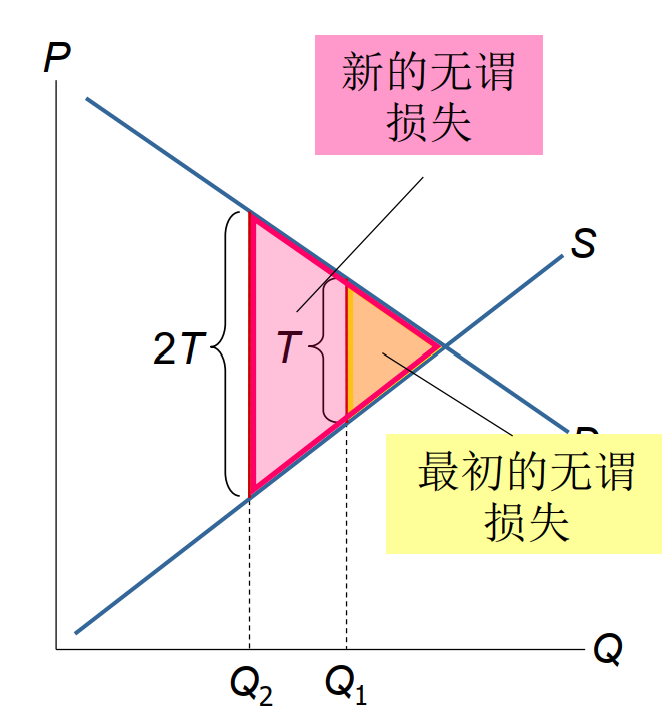
\includegraphics[width=0.4\textwidth]{税收规模与无谓损失.png} 
  \caption{税收规模增长速度比无谓损失的增长速度小} % 为图片添加标题
\end{figure}

含义:当税率低时,提高或降低税率既不会带来太大的损失,也不会带来太多的好处;当税率高时,提高税率的损失非常大,而降低税率的好处也非常明显
\begin{figure}[H] 
  \centering % 使图片居中显示
  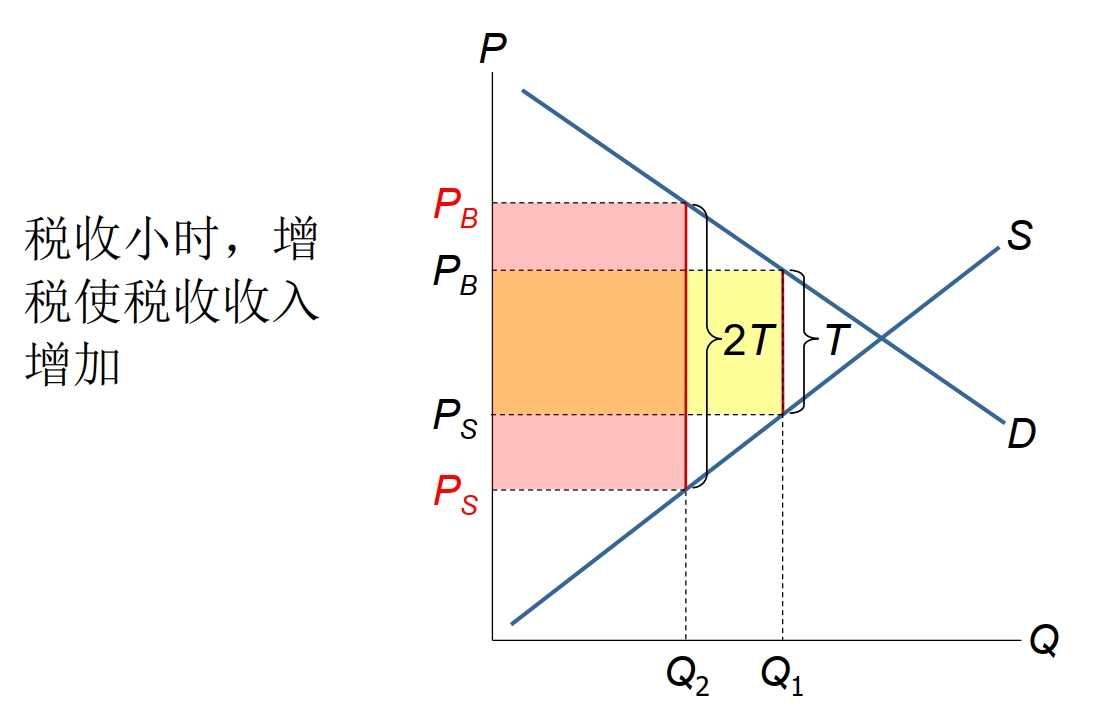
\includegraphics[width=0.5\textwidth]{税收小.png} 
  \caption{税收小,增税使税收收入增加} % 为图片添加标题
\end{figure}
\begin{figure}[H] 
  \centering % 使图片居中显示
  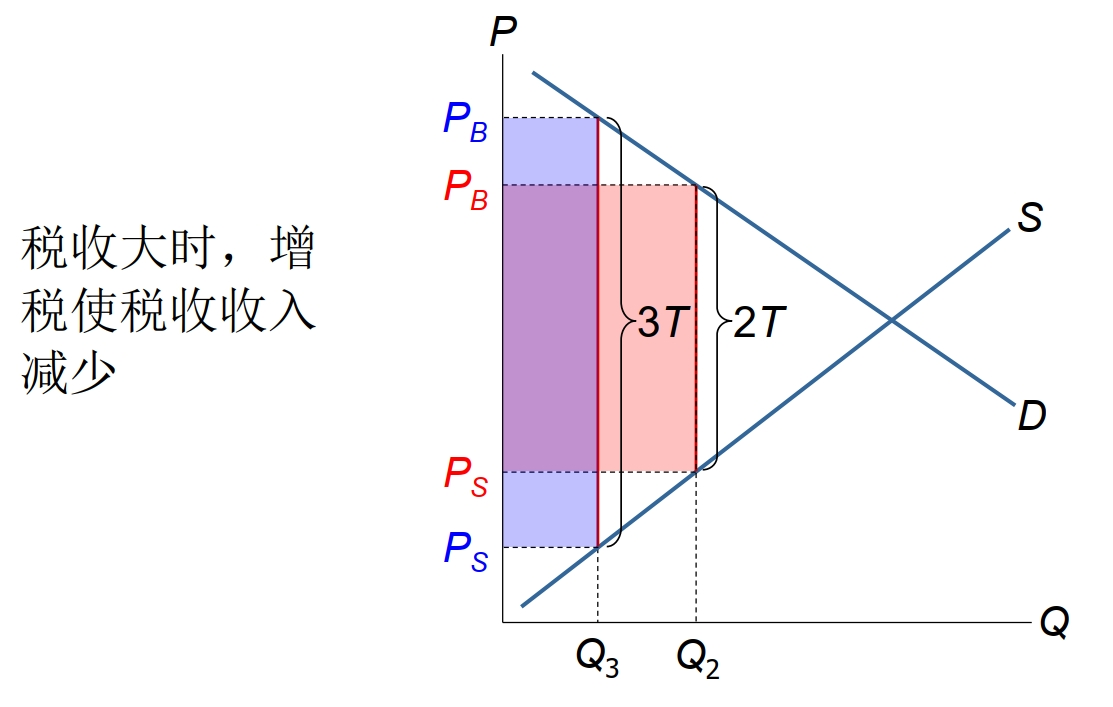
\includegraphics[width=0.5\textwidth]{税收大.png} 
  \caption{税收大,增税使税收收入减少} % 为图片添加标题
\end{figure}
\begin{figure}[H] 
  \centering % 使图片居中显示
  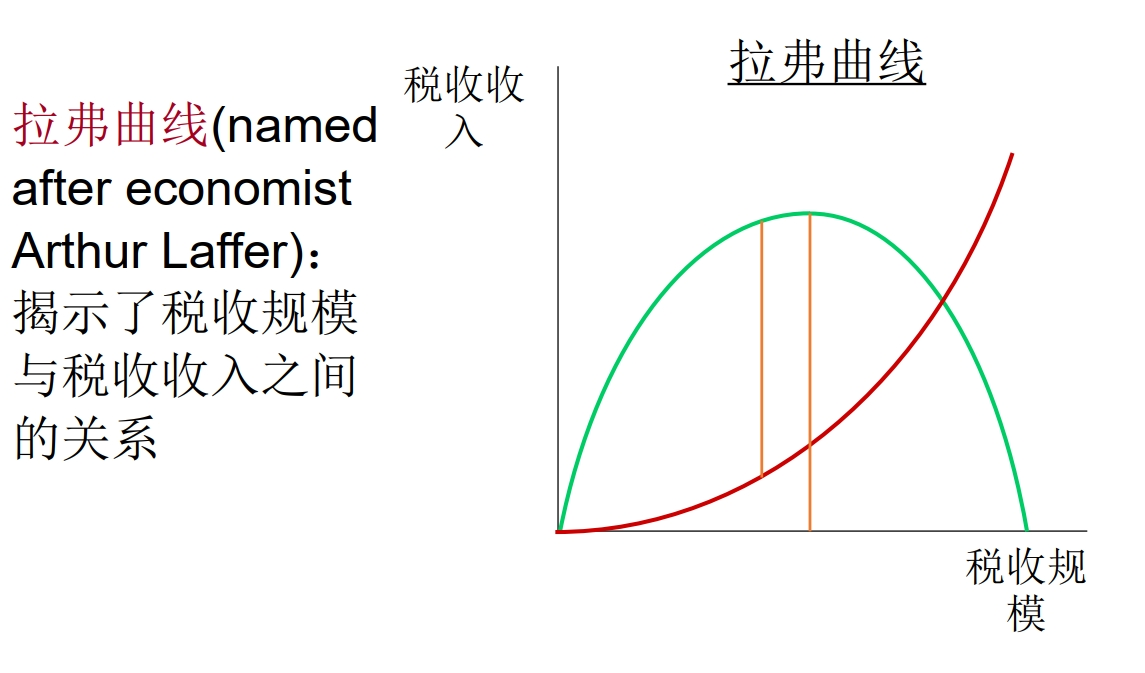
\includegraphics[width=0.5\textwidth]{拉弗曲线.png} 
  \caption{拉弗曲线} % 为图片添加标题
\end{figure}

\newpage
%Chapter 6外部性
\section{外部性}
\setstretch{1.5}

% 6.1
\subsection{外部性和市场无效率}
\textcolor{red}{外部性}指一个人的行为对旁观者福利的无补偿影响。

外部性有负外部性或正外部性之分,这取决于其对旁观者福利的影响是有利的还是不利的。

存在负外部性时,市场均衡数量大于社会合意的数量。

存在正外部性时,市场均衡的数量小于社会合意的数量。

为了解决问题,可以使外部性内在化,使价格等于社会成本。对负外部性的物品征税,对正外部性的物品补贴。

%6.1.1负外部性
\subsubsection{负外部性}
负外部性对旁观者福利有不利影响。例如,煤炭生产会排放污染物,损害周围居民的健康。

\textcolor{red}{社会成本}等于生产者私人成本加上受到污染的不利影响的旁观者的成本。

负外部性的社会成本在供给曲线(生产者私人成本)上方。

\begin{figure}[H]
  \centering
  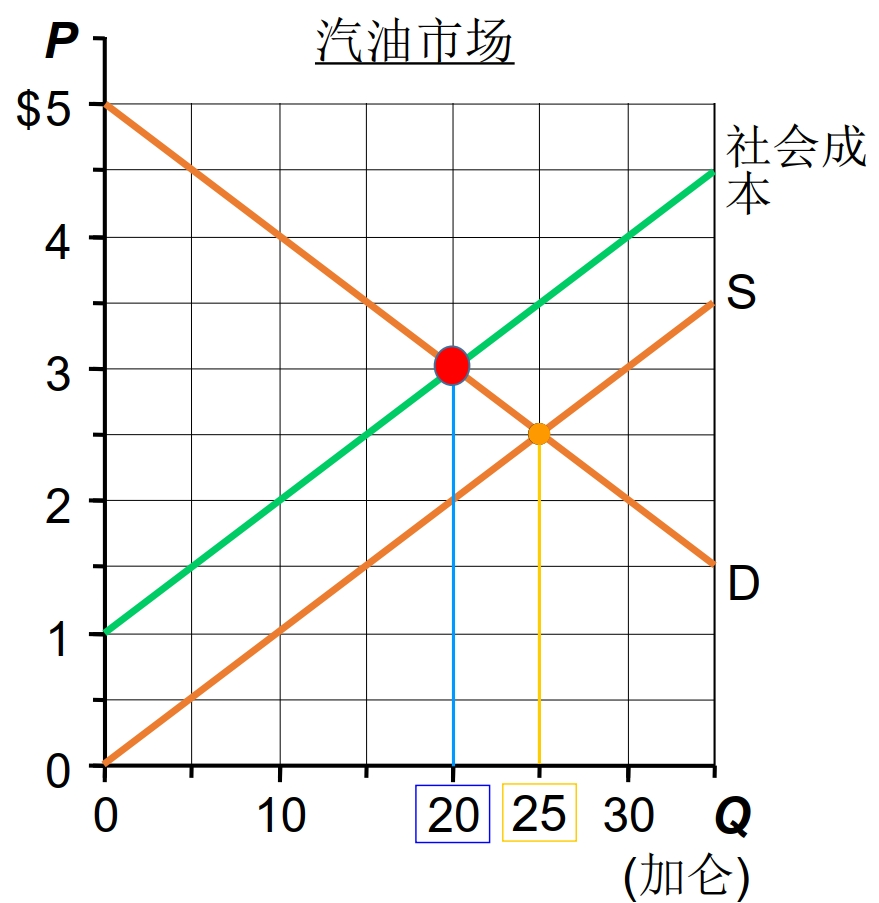
\includegraphics[width=0.4\textwidth]{负外部性.png}
  \caption{负外部性的社会成本}
\end{figure}

在有负外部性的情况下,市场总剩余并不是最大,因为最佳均衡点右侧的三角形面积是无谓损失(成本大于价值)。最佳生产量应当小于市场均衡量。

\textcolor{red}{外部性内在化}:改变激励,以使人们考虑到自己行为的外部效应。例如对卖者征税,使卖者成本等于社会成本。

当市场参与者必须支付社会成本时,市场均衡等于社会均衡。

%6.1.2正外部性
\subsubsection{正外部性}
正外部性对旁观者福利有利。例如,个人的教育可以为旁观者带来的有利影响。

社会价值等于私人价值加上教育为旁观者带来的有利影响的价值。

\begin{figure}[H]
  \centering
  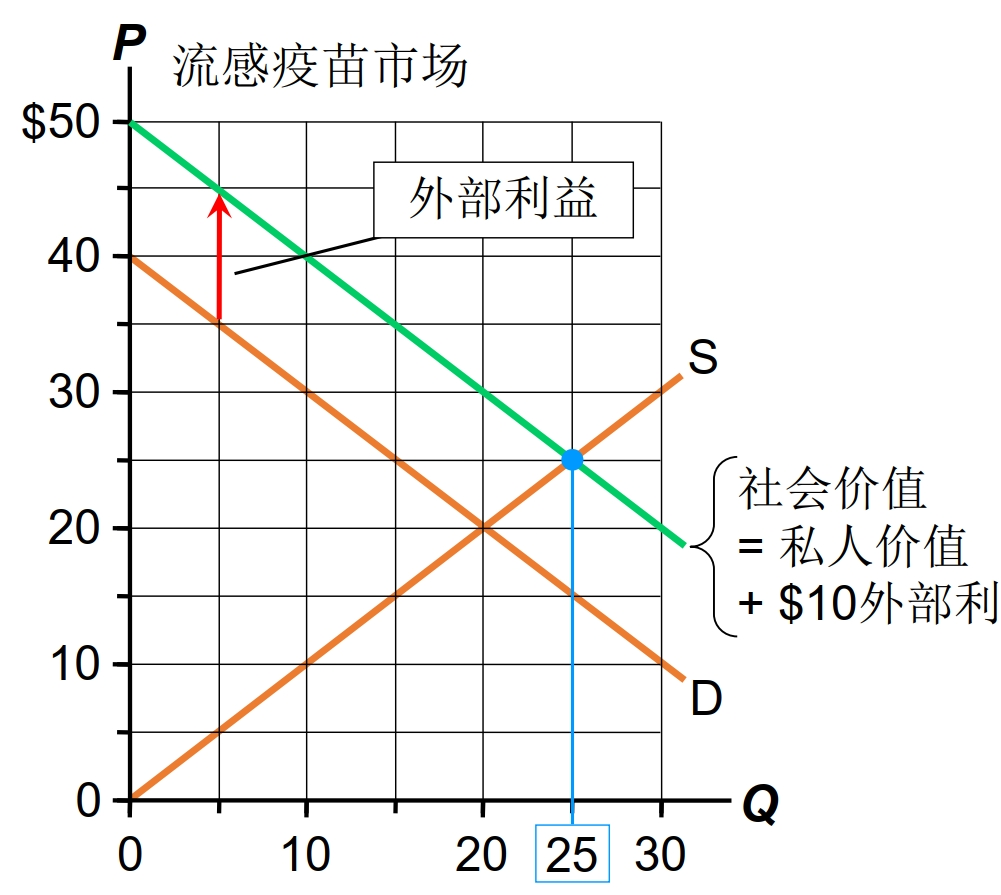
\includegraphics[width=0.4\textwidth]{正外部性.png}
  \caption{正外部性的社会成本}
\end{figure}

%6.2
\subsection{针对外部性的政府解决方法}
%6.2.1
\subsubsection{命令与控制政策:直接管制}
例如,限制排放的污染数量或强制企业采取某种技术来减少排放量,如限制每单位产出的排污量。

%6.2.2
\subsubsection{以市场为基础的政策 (market-based)}
向私人决策者提供激励,然后市场会自动矫正到最优数量。

\textbf{A. 矫正性税收与补贴}

矫正税,也被称为庇古税。理想的矫正税等于外部成本;理想的矫正补贴等于外部利益。

\textcolor{red}{难点:施加庇古税为什么可以做到没有无谓损失?}

矫正税通过增加生产成本,使得市场价格更加真实地反映了商品或服务的社会成本。这导致价格上升,从而减少了对具有负外部性商品或服务的需求,使得生产量降低到社会最优水平。

矫正税和其他税的影响不同。其他税收与补贴会扭曲激励,并使经济远离社会最优数量。而矫正性税收与补贴:

1. 使私人激励与社会的利益结合在一起。

2. 使私人决策者在做决策时考虑到他们行为的外部利益与外部成本。

3. 使经济向一个资源配置更有效率的方向移动。

矫正税/补贴的难点在于,外部成本与外部利益非常难以测量,很难确定政府的税收和补贴究竟是否合理。

\textbf{B. 可交易的污染许可证 (tradable permits)}

关键假设是企业的减排成本不同。

在市场均衡里,减排成本低的企业会减排,并出售他们的permit;减排成本高的企业更有动机购买permit(如果permit的价格低于减排成本)。

% 6.3 公共物品与公共资源
\subsection{公共物品与公共资源}
私人物品的特点是排他性(可以阻止一些人使用这个物品的特性)与竞争性(一个人使用该物品将减少其他人对它的使用的特性)。

\textcolor{red}{公共物品(public goods)}是既无排他性又无竞争性的物品。

公共物品由于搭便车问题,个人没有动机去提供,所以必须依靠政府。

\textcolor{red}{公共资源(public resources)}是没有排他性但具有竞争性的物品。

公共资源的使用具有负外部性,政府可以通过管制或税收政策来解决公地悲剧,但更好的方法可能是确定产权(将公共资源转化为私人产权)。


\newpage
%Chapter 7
\section{生产成本}

%7.1
\setstretch{1.5}
\subsection{生产与成本}
%7.1.1
\subsubsection{成本}
成本等于显性成本加上隐性成本。

\textcolor{red}{显性成本}:需要企业支出货币的投入成本。例如:支付给工人的工资。

\textcolor{red}{隐性成本}:不需要企业支付货币的投入成本。例如:企业所有者时间的机会成本。

经济利润与会计利润的区别可参考下图。

\begin{figure}[H]
  \centering
  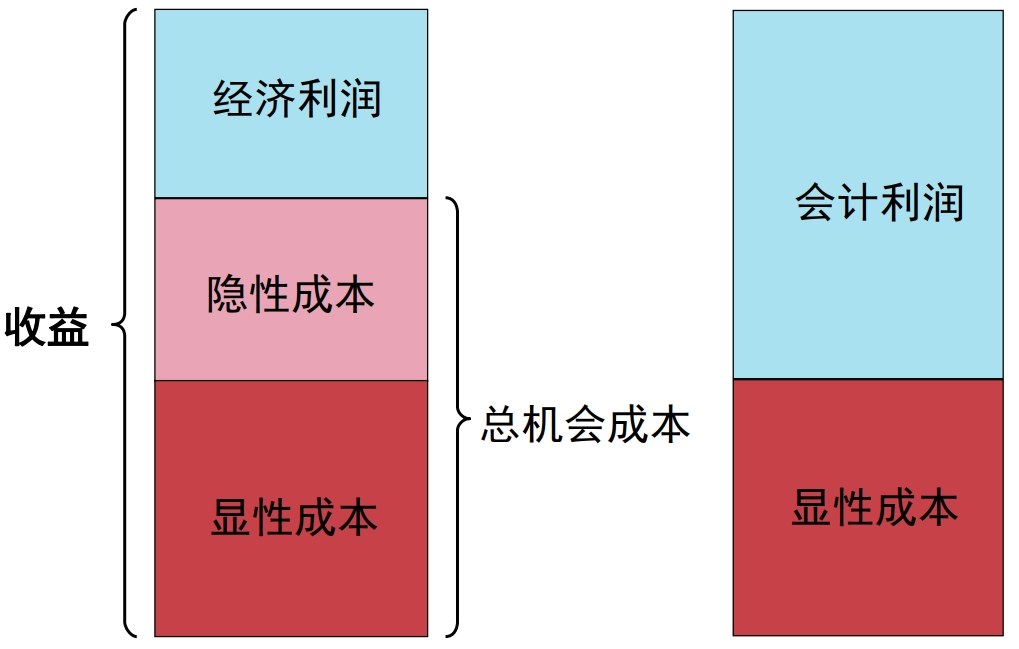
\includegraphics[width=0.4\textwidth]{经济利润与会计利润.png}
  \caption{经济利润与会计利润}
\end{figure}

%7.1.2
\subsubsection{生产函数}
\textcolor{red}{生产函数}:用于生产一种物品的投入量与该物品产量\( Q \)之间的关系。

\textcolor{red}{投入量(input)}:劳动力\( L \)加上资本\( K \)。
\( L \)代表劳动的时间和劳动的人数;\( K \)代表例如机器,厂房,土地等。

\[ Q = f(L, K) \]

产量\( Q \)的上限由资本\( K \)决定。

投入量可分为\textcolor{red}{可变投入量(variable input)}和\textcolor{red}{固定投入量(fixed input)}。前者容易改变(例如劳动时间),后者不容易改变(例如厂房的大小)。

\begin{figure}[H]
  \centering
  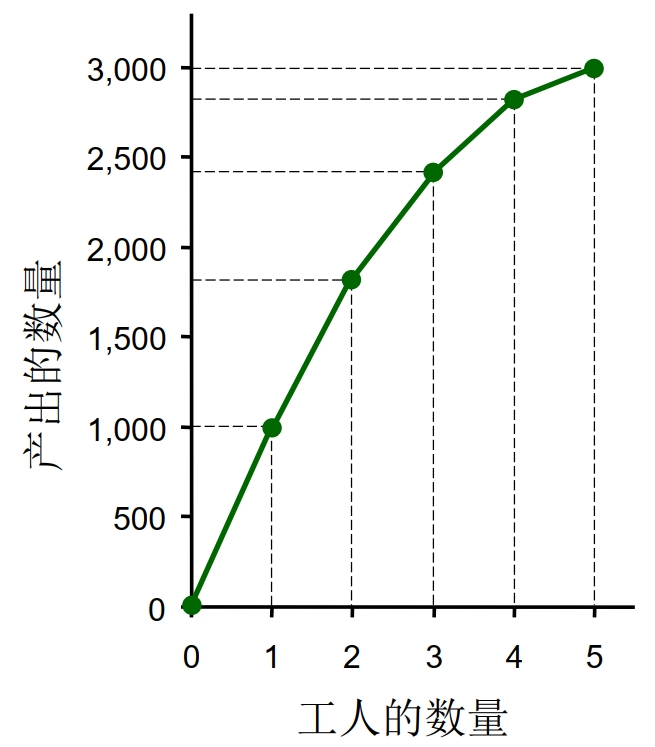
\includegraphics[width=0.4\textwidth]{生产函数.png}
  \caption{生产函数:越来越平坦(边际收益递减)}
\end{figure}

\textcolor{red}{投入的边际产量}:在其他投入量不变情况下,增加一单位投入所引起的产量增加。

设\( \Delta Q \)为产出的变动量,\( \Delta L \)为劳动的变动量。

\textcolor{red}{劳动的边际产量(生产函数的斜率)}定义如下:

\[ MP_L = \frac{\Delta Q}{\Delta L} \]

%7.2
\subsection{成本的衡量指标}

总成本\( TC \)分为固定成本和可变成本。

\textcolor{red}{固定成本(FC: fixed costs)}:不随着产量变动而变动的成本。例如设备成本,偿还贷款,租金支付——固定投入带来的成本。

\textcolor{red}{可变成本(VC: variable costs)}:随着产量变动而变动的成本。例如支付给工人的工资,原材料的成本——可变投入带来的成本。

\begin{figure}[H]
  \centering
  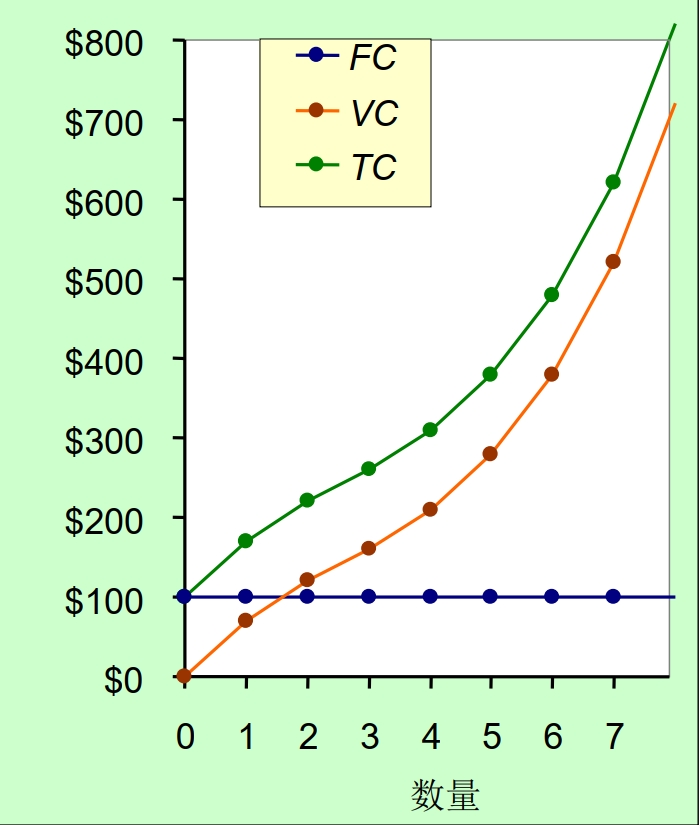
\includegraphics[width=0.3\textwidth]{成本函数.png}
  \caption{TC, FC, VC}
\end{figure}

\textcolor{red}{边际成本(MC: marginal costs)}:额外一单位产量所引起的总成本的增加定义如下:

\[ MC = \frac{\Delta TC}{\Delta Q} = \frac{\Delta VC}{\Delta Q} \]

边际成本是边际产量的倒数,且边际成本递增——斜率可能不变,也可能递增。

\textcolor{red}{平均总成本(ATC)}:平均固定成本加上平均可变成本。告诉我们总成本在所生产的所有单位中平均分摊,即平均一单位产品的成本。

\[ ATC = \frac{TC}{Q} = AFC + AVC \]

\begin{figure}[H]
  \centering
  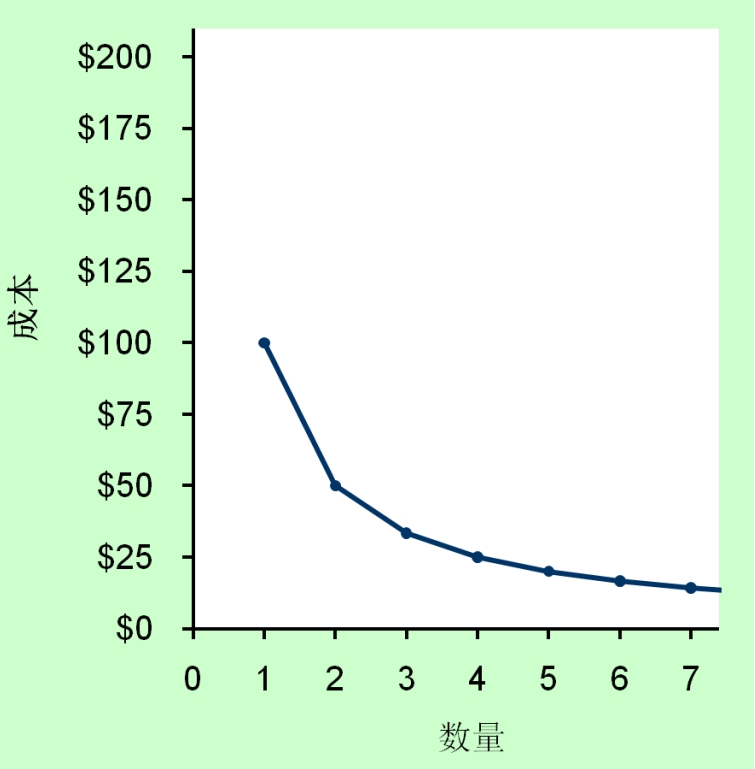
\includegraphics[width=0.4\textwidth]{AFC.png}
  \caption{平均固定成本(AFC)}
\end{figure}

\begin{figure}[H]
  \centering
  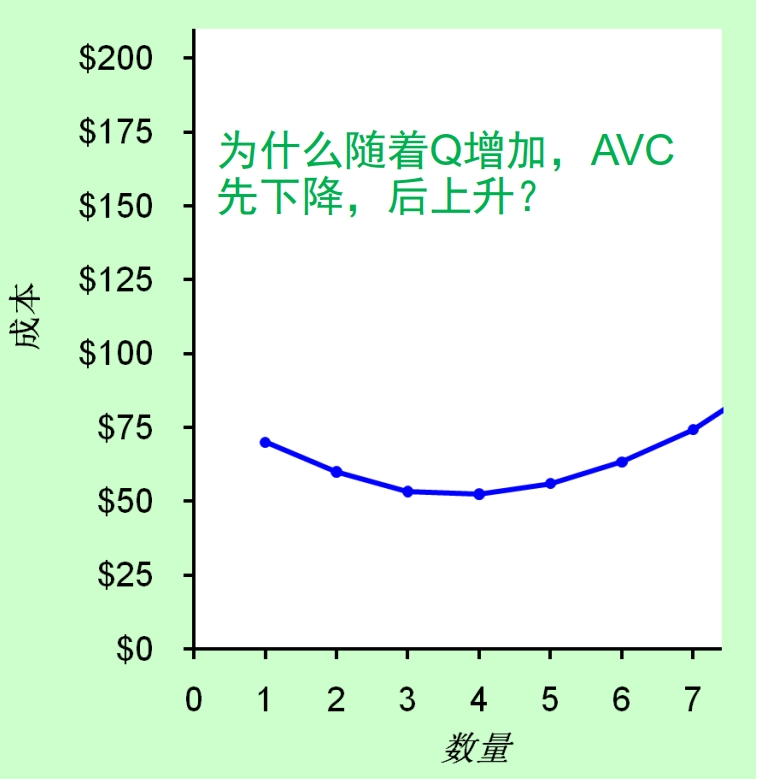
\includegraphics[width=0.4\textwidth]{AVC.png}
  \caption{平均可变成本(AVC)}
\end{figure}

随着产量增加,平均可变成本先下降后上升。

\begin{figure}[H]
  \centering
  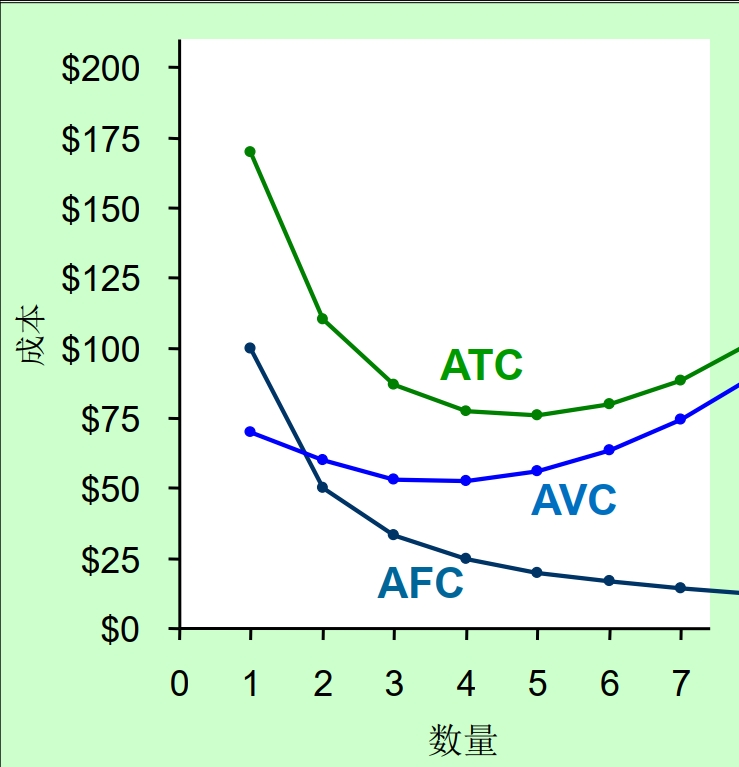
\includegraphics[width=0.4\textwidth]{ATC.png}
  \caption{平均总成本(ATC):U形}
\end{figure}

平均总成本曲线是U形。U形曲线的低端是企业的 \textbf{有效规模——使平均总成本最小的产量}。

\begin{figure}[H]
  \centering
  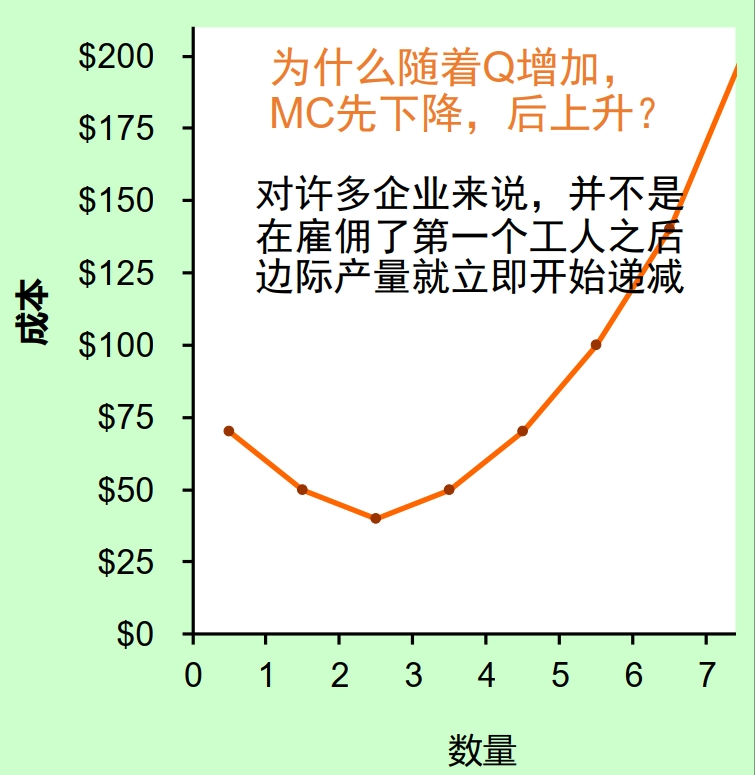
\includegraphics[width=0.4\textwidth]{MC.png}
  \caption{边际成本(MC)}
\end{figure}

\begin{figure}[H]
  \centering
  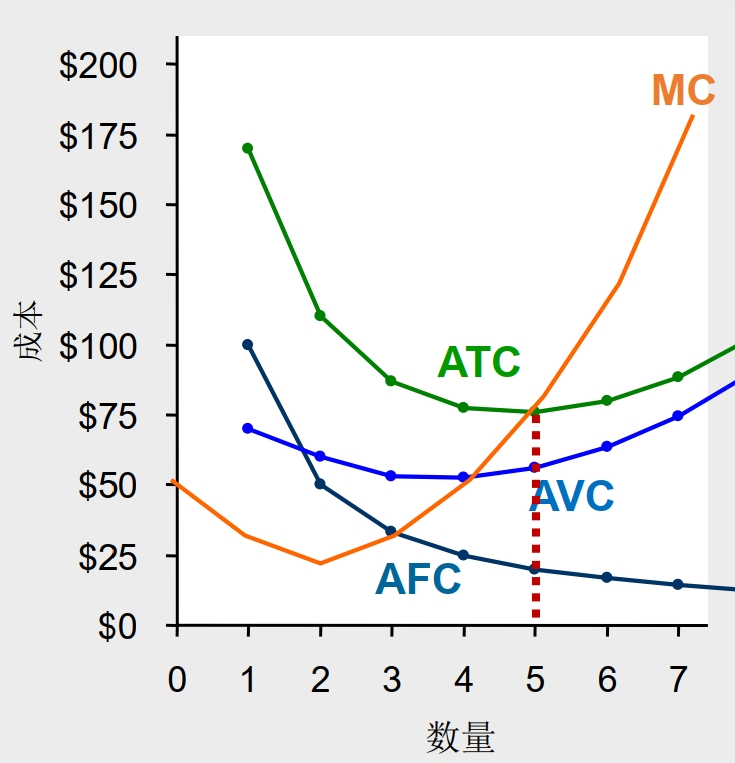
\includegraphics[width=0.4\textwidth]{各种成本曲线.png}
  \caption{各种成本曲线}
\end{figure}

当\( MC < ATC \),则\( ATC \)减少;当\( MC > ATC \),则\( ATC \)增加。

MC曲线从ATC曲线的最低点处穿过。

企业的各种成本包括:总成本、固定成本、可变成本;平均总成本、平均固定成本、平均可变成本、边际成本;以及边际成本从平均总成本和平均可变成本的最低点穿过;平均总成本最低的点对应的数量是企业的有效规模。

\[ ATC = \frac{TC + \Delta TC}{Q + \Delta Q} \]
\[ AVC = \frac{VC + \Delta VC}{Q + \Delta Q} \]
\[ MC = \frac{\Delta TC}{\Delta Q} = \frac{\Delta VC}{\Delta Q} \]

平均总成本最低的点对应的数量是企业的有效规模 (efficient scale)

%7.3
\subsection{短期成本与长期成本}
%7.3.1
\subsubsection{短期与长期}

\begin{description}
  \item[短期 (SR: short run):] 一些投入的数量是固定的(比如,工厂,土地)。这些投入的成本是固定成本。
  \item[长期 (LR: long run):] 所有投入的数量都是可变的(比如,企业可以建造更多的工厂或者出售已建好的工厂)。在长期里,任何企业的产量都被调整为有效规模 — 即平均总成本最小的规模。
  \item[\textcolor{red}{长期平均总成本(LATC):}] 在任何低于QA的产量,企业在长期会选择规模 S;生产在QA与QB之间的产量,企业在长期会选择规模M;生产高于QB的产量,企业在长期会选择规模L 
\end{description}


\begin{figure}[H] 
  \centering % 使图片居中显示
  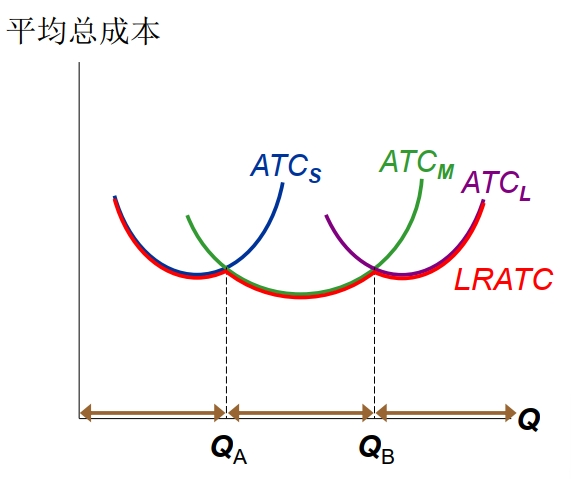
\includegraphics[width=0.4\textwidth]{长期平均总成本.png} 
  \caption{长期平均总成本曲线(LRATC)} % 为图片添加标题
\end{figure}

%7.3.2
\subsubsection{规模经济}

ATC沿LRATC变动的三个阶段:随Q增加,ATC下降、不变、增加。

\begin{itemize}
  \item \textcolor{red}{规模经济 (increasing return to scale)}:长期平均总成本随产量增加而减少。 
  
  产生原因是较高的产量水平允许工人实现专业化,例如,专业化可以使工人更精通某一项工作,如流水线上的工人。 
  
  通常在产量低时,规模经济更常见。

  \item \textcolor{red}{规模收益不变 (constant return to scale)}:长期平均总成本在产量变动时保持不变。

  \item \textcolor{red}{规模不经济 (decreasing return to scale)}:长期平均总成本随产量增加而增加。 
  
  规模不经济的产生是由于任何一个大型组织中固有的协调问题,例如,管理团队越庞大,管理协调困难;中央计划等。
\end{itemize}


\newpage
% Chapter 8
\section{竞争市场}

\subsection{什么是竞争市场}

\textcolor{red}{完全竞争市场的特点}:

\begin{itemize}
  \item 企业数量:非常多,每个企业都是价格接受者,单独的企业对市场价格没有影响。

  \item 价格:由市场均衡决定,企业只能接受市场价格。

  \item 产品同质性:产品完全相同,消费者认为所有企业的产品是完全可替代的。
  
  \item 市场进入和退出:非常自由,没有障碍。新企业可以轻易进入市场,不成功的企业可以自由退出。
\end{itemize}

\subsection{利润最大化}

\subsubsection{\textbf{竞争企业的各种收益}}

\[ TR (Total Revenue) = PQ \]

\[ AR (Average Revenue) = \frac{TR}{Q} = P \]

\[ MR (Marginal Revenue) = \frac{d(TR)}{d(Q)} = P\]

当销售额增加一个单位时,由于企业不能影响价格,总收入增加的额度正好等于该商品的市场价格

\[ \textcolor{red}{AR = MR} \]

\subsubsection{竞争企业的利润最大化:通过选择最优的产量}

\[pi(q) = TR(q) - TC(q)\]

产量增加一单位,收益增加MR,成本增加MC

如果 MR > MC,那增加产量会提高利润

如果MR < MC,那降低产量会提高利润

增加产量直到 MR = MC (MC一般是递增的,后期q增加会使MC超过MR)

\textbf{MR = MC 时的产量是利润最大化的产量}

\begin{figure}[H] 
  \centering % 使图片居中显示
  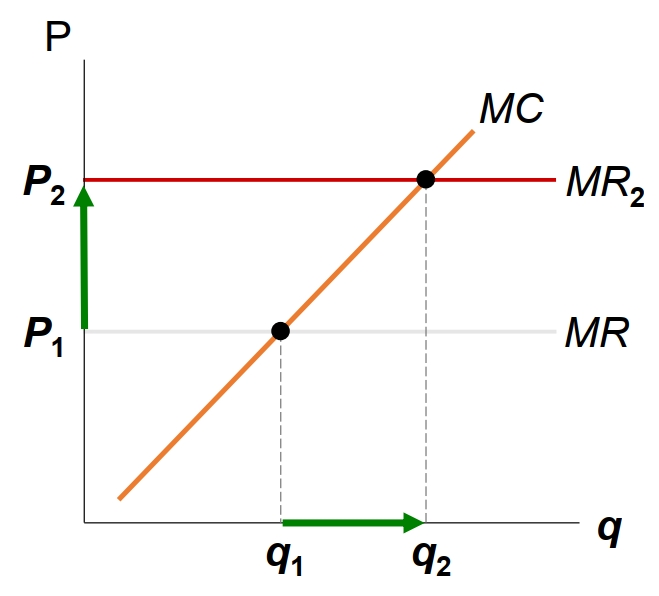
\includegraphics[width=0.4\textwidth]{完全竞争市场的企业利润最大化.png} 
  \caption{边际成本与企业的供给决策} % 为图片添加标题
\end{figure}

MC 曲线决定了企业在任何一种价格下愿意提供的物品数量

\textbf{因此,MC 曲线便是每个企业的供给曲线}



\subsection{企业的短期停止营业与长期退出市场}

\subsubsection{企业的短期决策:停止营业}

\begin{itemize}
  \item 沉没成本: 已经发生而且无法收回的成本  e.g. 已支付的房租、购买的设备、资金的opportunity cost

  \item 停止营业的成本:收益损失 = TR

  \item 停止营业的收益:节约成本 = VC (企业仍然必须支付 FC)

  \item 因此,如果 TR < VC ,停止营业

  \item 等式两边除以产量: TR/q < VC/q
  
  \item 因此,企业停止营业的标准是:如果 P < AVC, 停止营业
\end{itemize}

\begin{figure}[H] 
  \centering % 使图片居中显示
  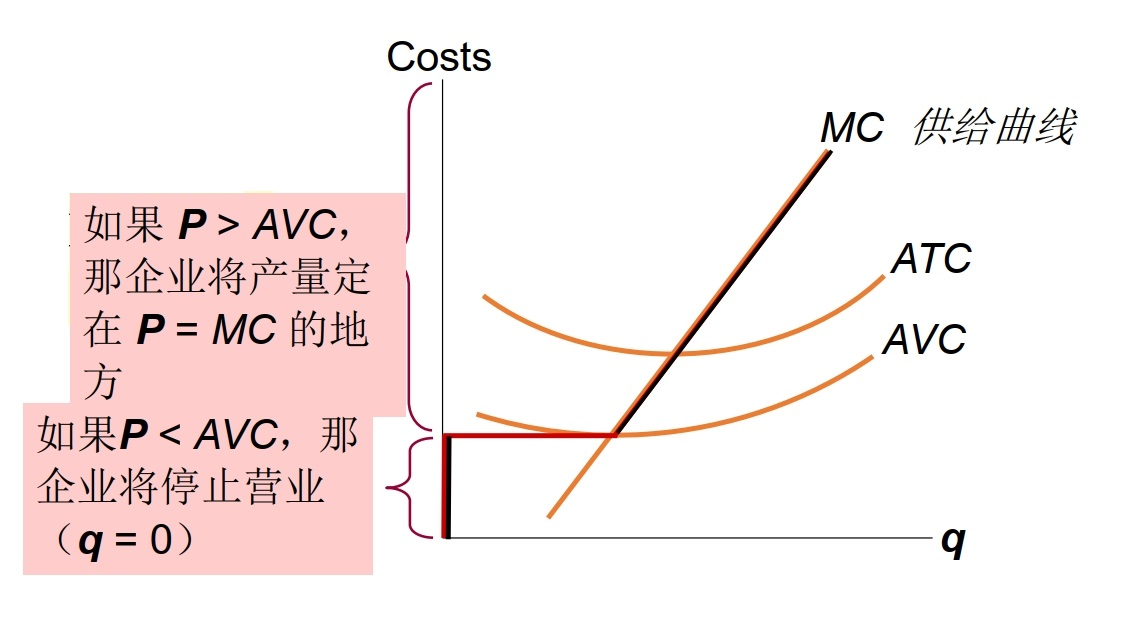
\includegraphics[width=0.5\textwidth]{短期决策.png} 
  \caption{短期竞争企业的供给曲线} % 为图片添加标题
\end{figure}

\subsubsection{企业的长期决策:退出市场}

\begin{itemize}
  \item 退出市场的成本:收益损失 = TR

  \item 退出市场的收益:节约成本 = TC (长期内固定成本为0)

  \item 因此,如果 TR < TC ,企业退出市场

  \item 等式两边除以产量:如果 P < ATC,退出市场
\end{itemize}

\subsubsection{企业的长期决策:进入市场}

长期内,如果 TR > TC, 一个新企业将进入市场

等式两边除以产量:如果 P > ATC,进入市场

\begin{figure}[H] 
  \centering % 使图片居中显示
  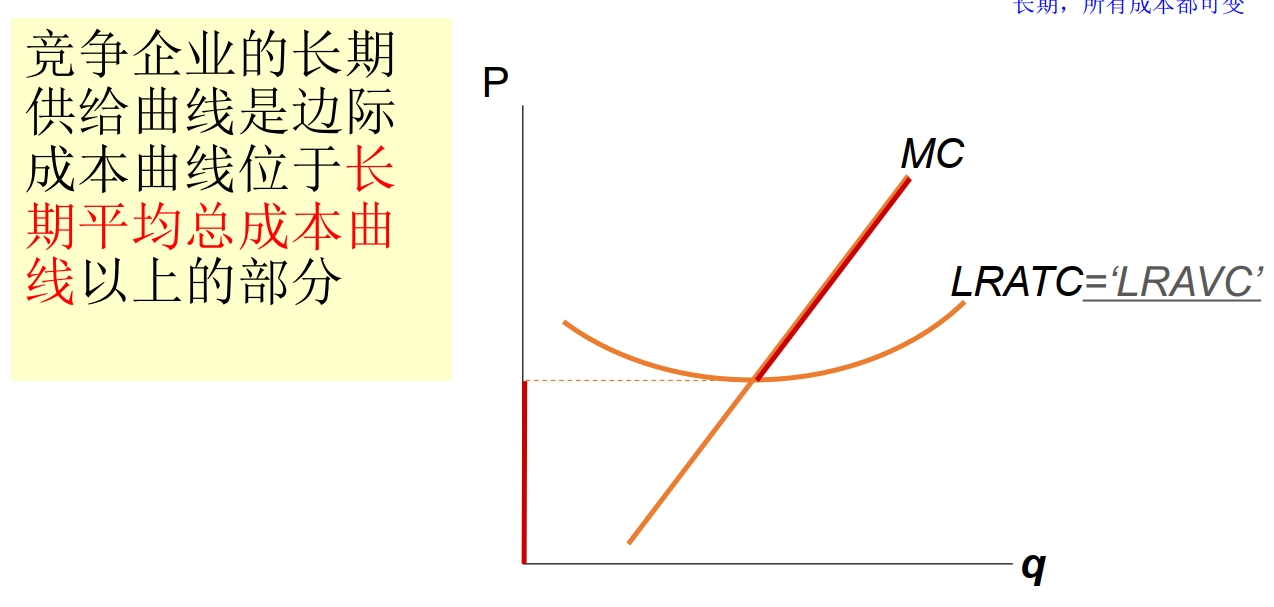
\includegraphics[width=0.5\textwidth]{长期供给曲线.png} 
  \caption{长期竞争企业的供给曲线} % 为图片添加标题
\end{figure}
因为在长期中,企业可以调整所有成本,所有成本都可变,所以LRATC=LRAVC

\subsubsection{竞争企业的利润}

竞争企业的利润:价格和平均总成本之间的面积

\begin{figure}[H] 
  \centering % 使图片居中显示
  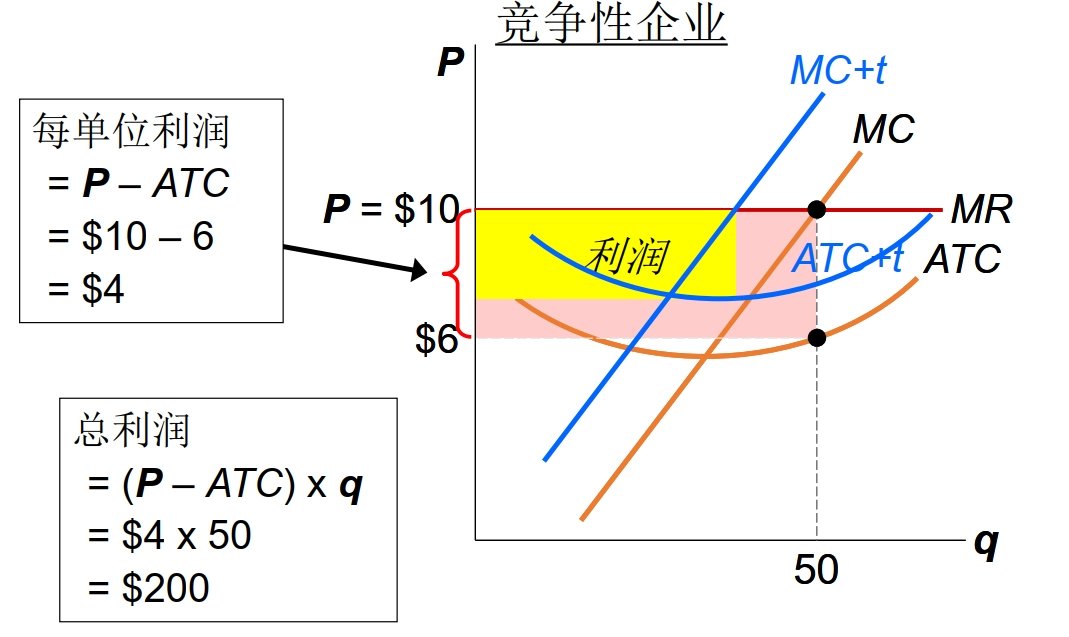
\includegraphics[width=0.5\textwidth]{竞争企业的利润.png} 
  \caption{竞争企业的利润} % 为图片添加标题
\end{figure}

竞争企业的损失:价格和平均总成本之间的面积

\begin{figure}[H] 
  \centering % 使图片居中显示
  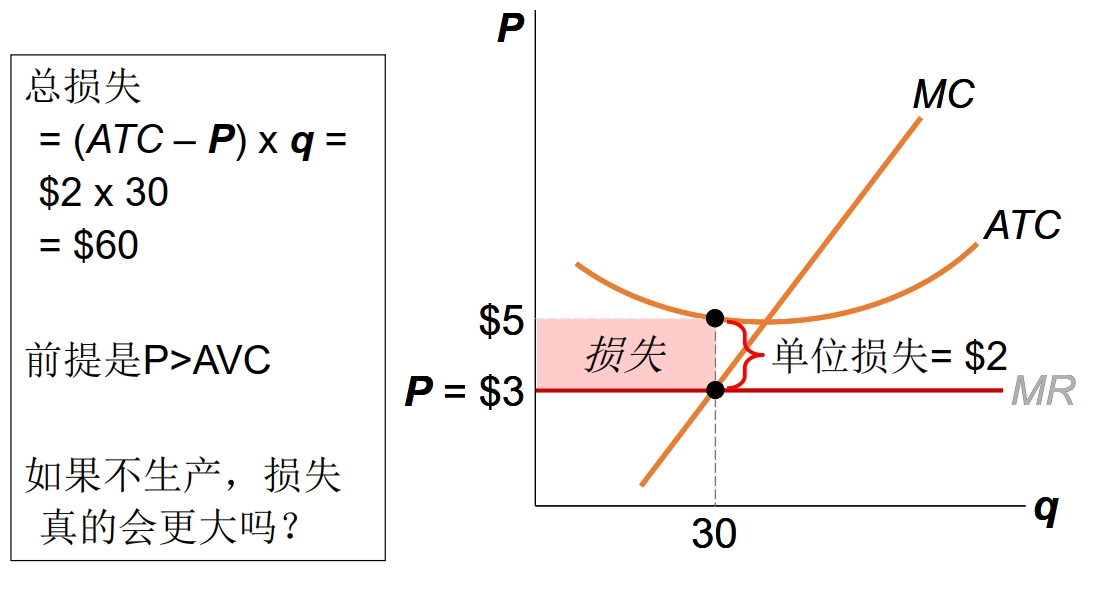
\includegraphics[width=0.5\textwidth]{竞争企业的损失.png} 
  \caption{竞争企业的损失} % 为图片添加标题
\end{figure}

\subsection{竞争市场中的供给曲线}

\subsubsection{短期竞争市场的供给}

假设:

\begin{itemize}
  \item 所有市场上的企业与市场的潜在进入者都有相同的成本

  \item 一些企业进入或退出市场并不影响另外一些企业的成本

  \item 市场中企业的数量: 短期内固定(由于固定成本;长期内可变(由于进入与退出市场都无限制)
\end{itemize}

只要 P ≥ AVC, 每个企业都将生产利润最大化的产量,也就是在 MR = MC = P时的产量

在每个价格上的市场供给量Q是这个价格时所有企业的供给量q的总和

\begin{figure}[H] 
  \centering % 使图片居中显示
  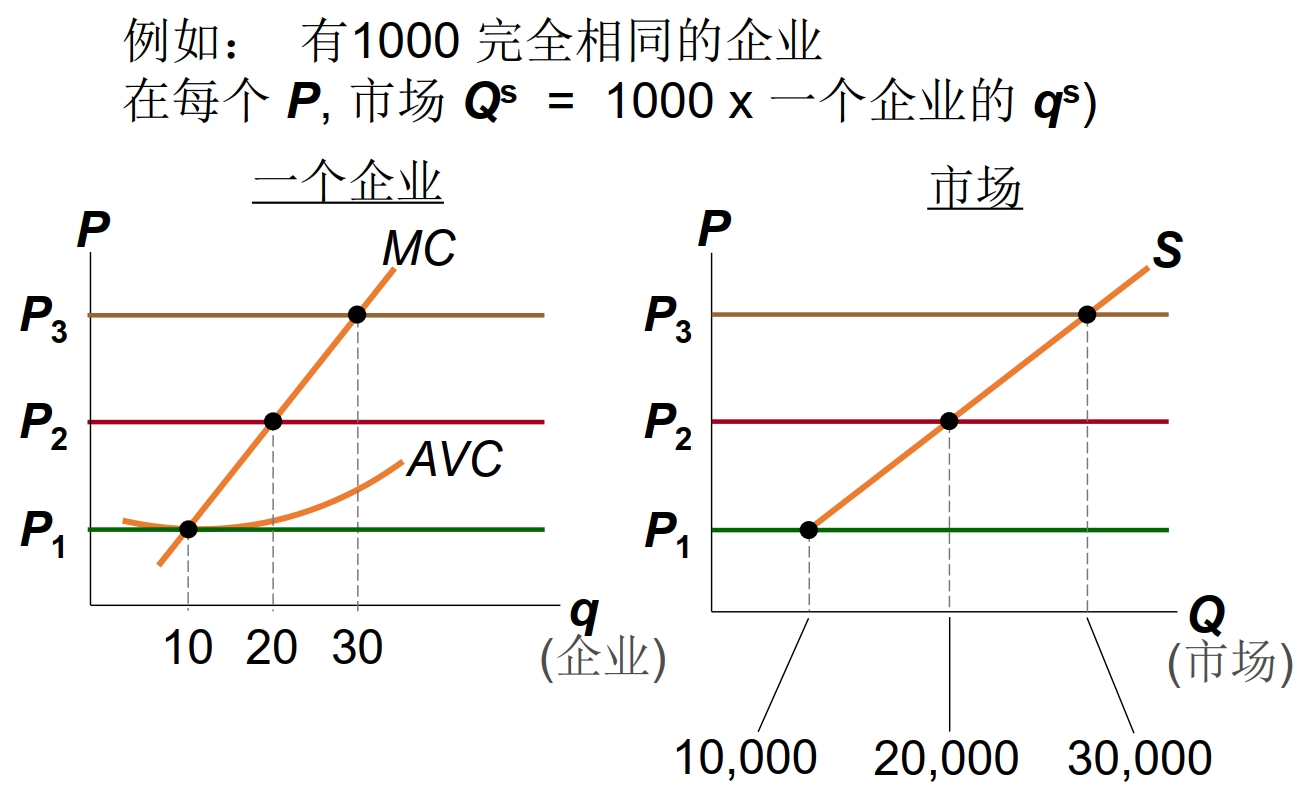
\includegraphics[width=0.5\textwidth]{短期市场供给曲线.png} 
  \caption{短期市场供给曲线:P在AVC以上部分的MR曲线} % 为图片添加标题
\end{figure}

\subsubsection{长期市场供给曲线}
在长期中,由于企业的进入与退出,企业数量会发生变化。

假设:
\begin{itemize}
    \item 在长期内,所有成本都是可变的。
    \item 平均总成本(ATC)的最小化:在长期内,企业可以调整规模,以达到平均总成本最小化的生产水平。这个最小点称为最低平均总成本(minATC)。
\end{itemize}

长期市场均衡的调整:
\begin{itemize}
    \item 如果市场上的企业获得正的经济利润(价格高于minATC):
    \begin{itemize}
        \item 新企业会进入,短期市场供给向右移动。
        \item 价格下降,利润降低,企业进入速度减慢。
    \end{itemize}
    \item 如果市场上的企业有亏损(如果价格低于minATC):
    \begin{itemize}
        \item 一些企业会退出市场,短期市场供给向左移动。
        \item 价格上升,减少仍在市场上企业的损失。
    \end{itemize}
\end{itemize}

长期均衡:
\begin{itemize}
    \item 在进入和退出过程结束时,仍然留在市场中的企业的经济利润必定为零。
    \item 经济利润为零 $\rightarrow$ P=ATC。
    \item 由于企业在 MR = P = MC 处生产 $\rightarrow$ \textbf{P = MC = ATC}。
    \item MC 曲线只有在 ATC 曲线的最低点与 ATC 曲线相交(\textcolor{red}{有效规模})。
    \item 因此,在长期,P = minATC,且每一个企业都在有效规模 q* 上生产。
    \item 在这种均衡条件下,市场上的企业在任何给定的价格(等于minATC)上都能盈利地生产。因此,市场供给曲线在这个价格上是完全弹性的,即供给量可以在这一价格水平上无限量地增加或减少,而价格保持不变。这就是为什么长期供给曲线在完全竞争市场中是水平的。
    \item \textbf{长期均衡中没有无谓损失:$P = MC \leftrightarrow DWL = 0$}
\end{itemize}

\begin{figure}[H]
    \centering
    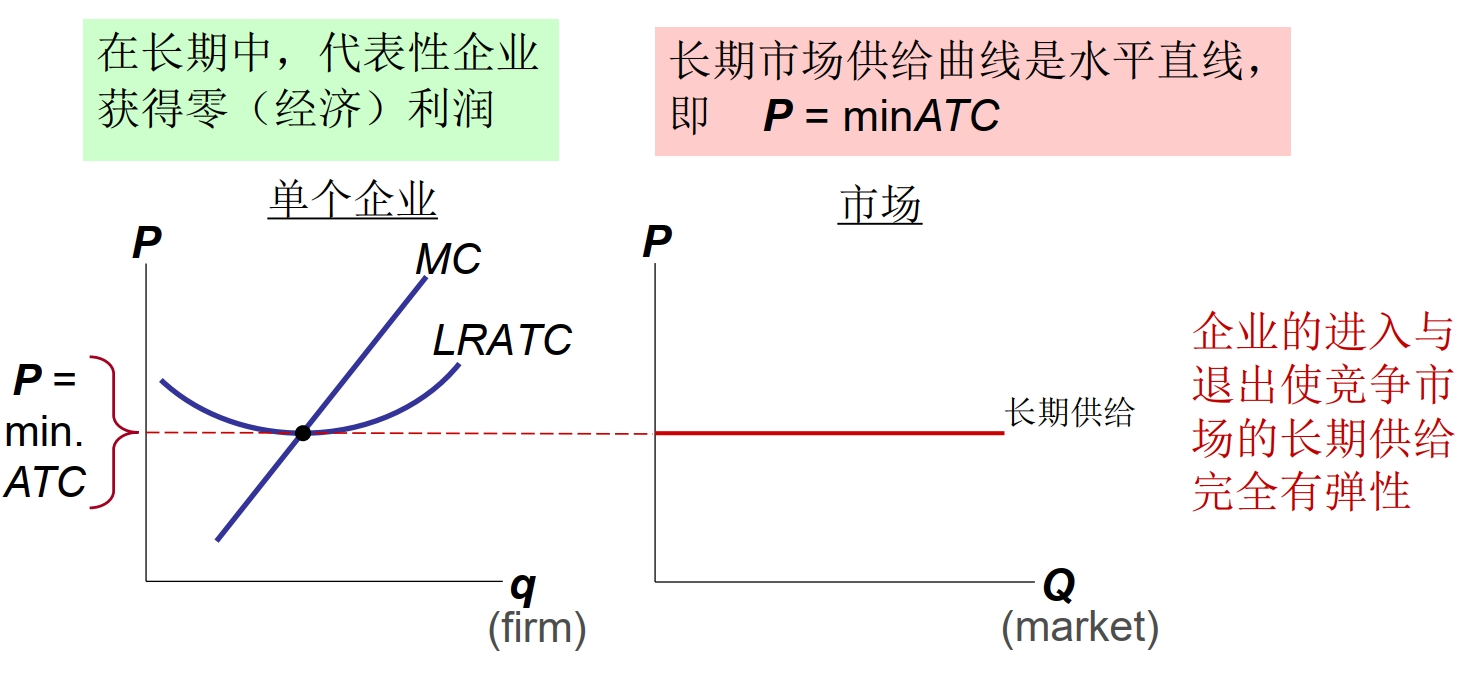
\includegraphics[width=0.5\textwidth]{长期竞争市场供给曲线.png}
    \caption{长期市场供给曲线}
\end{figure}

结论:
\begin{itemize}
  \item 当你向一个竞争市场中的企业购买产品时,可以保证你支付的价格接近生产该产品的成本
  \item 如果企业可以自由地进入和退出市场,价格还等于最低的平均生产总成本ATC → 在长期里,每个企业都在其有效规模上运营
  \item 在竞争市场中,虽然价格对企业是既定的,但本质上价格是由企业的成本决定的。需求的变化在长期里不会影响价格,只会影响数量
  \item 企业的成本往往是由技术(technology)决定的→竞争市场上,是科技与创新决定了消费者购买产品的价格与相关的社会的福利
\end{itemize}

\subsection{完全竞争市场的需求曲线}
在完全竞争市场,由于企业总是以既定的市场价格出售产品
一家竞争企业面临的需求曲线是水平的 MR = P

\newpage

% Chapter 9
\section{垄断和垄断竞争市场}

\subsection{什么是垄断}
如果一个企业是其产品唯一的卖者,而且其产品没有相近的替代品,那么这个企业就是一个垄断企业

垄断产生的原因:
\begin{itemize}
  \item 进入壁垒
  \begin{itemize}
    \item 生产所需要的关键资源由单个企业所拥有
    \item 政府给予单个企业排他性生产某种物品或劳务的权利
    \item 自然垄断:一个企业能能够以低于其他企业的成本向整个市场供应(往往是由于规模经济)
    \begin{itemize}
      \item 固定成本很大,而边际成本很小,从而在市场上,平均总成本总是在下降
      \item 现有企业的ATC<新进入者的ATC,存在进入门槛
    \end{itemize}    
  \end{itemize}
\end{itemize}

垄断与完全竞争市场的区别:

\begin{itemize}
  \item 垄断企业具有市场势力,是价格的制定者
  \item 一个竞争性企业则没有市场势力,只能接受市场价格
\end{itemize}

\subsection{垄断者的生产与定价决策}




\subsection{广告}

\newpage
% Chapter 10
\section{寡头市场}

\subsection{寡头市场与博弈论}

\subsubsection{寡头}

\textcolor{red}{寡头:只有少数几个卖者提供相同/相似产品的市场结构}

e.g. 石油公司、移动通讯公司

因此,市场上任何一个卖者的行为对其他企业的利润有很大影响。每一家企业都知道,它的利润不仅取决于他生产多少,还取决于其他企业生产多少。

\subsubsection{博弈论}

博弈论(Game Theory)帮助我们理解寡头企业之间如何相互影响,以及它们如何做决策

\begin{itemize}
  \item 囚徒困境:两个被捕的囚徒之间的一种特殊“博弈”,说明为什么在合作对双方都有利时,保持合作也是困难的。
  \item 对两人而言,坦白是占优策略。如果两人都不坦白,他们将更好。但自利的逻辑仍会起主导作用,合作破裂。
  \item 纳什均衡:两人都认罪
  
  \begin{figure}[H] 
    \centering % 使图片居中显示
    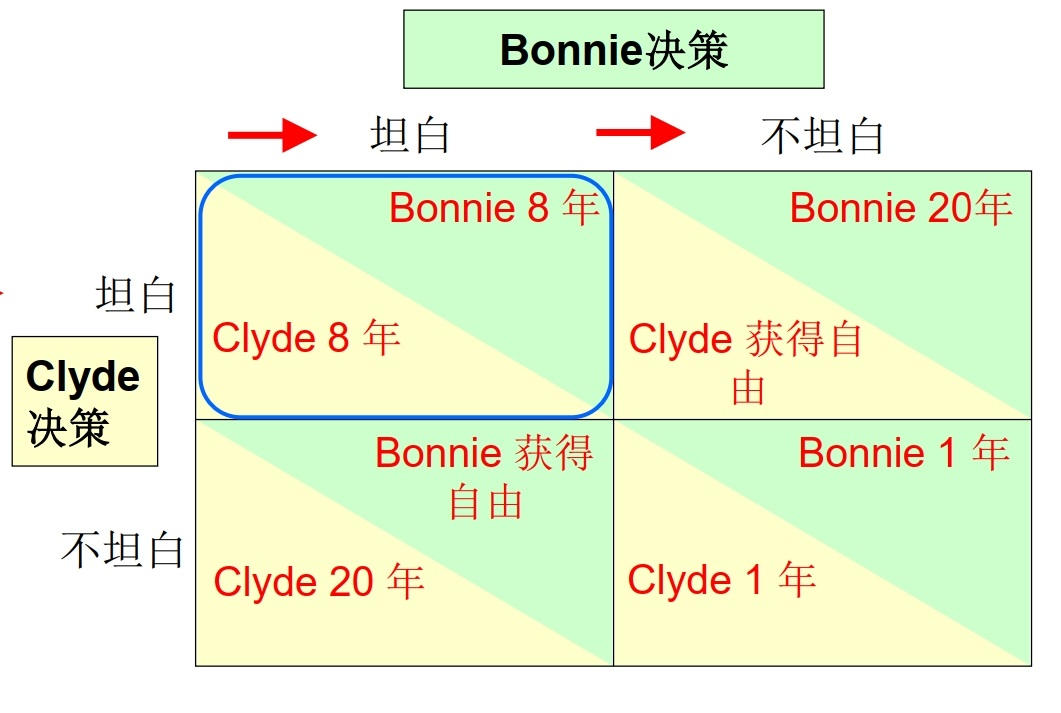
\includegraphics[width=0.5\textwidth]{囚徒困境.png} 
    \caption{囚徒困境} % 为图片添加标题
  \end{figure}


\end{itemize}

\newpage
% Chapter 11
\section{宏观经济学的数据}

\subsection{什么是宏观经济学}
\begin{itemize}
  \item 微观经济学(microeconomics):研究经济活动中个体(企业或家庭)的行为及后果
  \item 宏观经济学(macroeconomics):研究一国的整体经济运行及政府运用经济政策来影响经济运行
\end{itemize}

\begin{figure}[H]
  \centering
  \includegraphics[width=0.5\textwidth]{微观经济学vs宏观经济学.png}
  \caption{微观经济学vs.宏观经济学}
\end{figure}

\subsection{一国收入(经济总量)的衡量}
\textcolor{red}{国内生产总值(Gross Domestic Product GDP)}: 在某一既定时期\textbf{一个国家内生产}的所有最终物品与劳务的市场价值。

什么不包括在GDP之内?e.g.家里生产和消费而没有进入市场的大多数商品和服务;非法生产和销售的项目,如毒品。
\begin{itemize}
  \item “…最终…”:GDP只包括最终物品的价值,而不包括中间品的价值(价值只能计算一次)
  \item “…物品与劳务…”:它既包括有形的物品,也包括无形的劳务
  \item “…生产的…”:它包括现期生产的物品与劳务,并不包括涉及过去生产的东西的交易
  \item “…一个国家之内的…”:它衡量的生产价值是在一个国家的地理范围之内
  \item “…在某一既定时期内…”:它衡量某一既定时期内进行的生产的价值,通常这个时期是一年和一个季度
\end{itemize}

其他收入衡量指标:
\begin{itemize}
  \item 国民收入总值 Gross National Product (GNP):是一国永久居民(称为国民)所赚到的总收入 
  \item 国民生产净值 Net National Product (NNP):是一国居民的总收入减去折旧的消耗; 折旧是经济中设备和建筑物存量的磨损或损耗
  \item 国民收入 National Income:是一国居民在物品与劳务生产中赚到的总收入
\end{itemize}

GDP的组成部分(支出法):包括了用于国内生产的物品和服务的所有支出形式:
\begin{itemize}
  \item Consumption (C) 消费(C)
  \item Investment (I) 投资(I)
  \item Government Purchases (G) 政府购买(G)
  \item Net Exports (NX) 净出口(NX)
\end{itemize}

GDP的组成部分:
\begin{itemize}
  \item 消费 (C):家庭除了购买\textbf{新住房}以外用于物品与劳务的支出
  \item 投资 (I) ≠ 金融当中的投资:指用于\textbf{资本设备、存货和建筑物}的支出,其中包括家庭用于购买新住房的支出。是对用于在未来生产物品与服务的物品的购买
\end{itemize}

\end{document}